\section{Data Cleaning}
\label{evt-sel:cleaning}
\paragraph{}
Lumiblocks in 2015 and 2016 data that fail the Good Run List are rejected in order to ensure that all detector components are operating correctly. In addition, the following data cleaning requirements are made:
\begin{itemize}
\item Events with problems in TileCal/LAr are removed;
\item Events that are affected by the recovery procedure for single event upsets in the SCT are removed;
\item Events that fail the jet cleaning procedure are removed. This is designed to exclude jets caused by detector noise, non-collision backgrounds and cosmic rays;
\item Incomplete events are removed.
\end{itemize}
The analysis also runs over the debug stream, no event passing the full signal selection is found.


%%%%%%%%%%%%%%%%%%%%%%%%%%%%%%%%%%%%%%%%%%%%%%%%%%%%%%%%%%%%%%%%%%%%%%%%%%%%%%%%%%%%%%%%%%
\section{Trigger}
\label{evt-sel:trig}
\paragraph{}
%See \href{https://arxiv.org/pdf/1611.09661.pdf}{6.4.3} 
Events in data and simulation are required to pass the lowest unprescaled large-$R$ jet trigger: \\
\verb|HLT_j360_a10_lcw| in 2015 and \verb|HLT_j420_a10_lcw|, where topo-cluster jets with local calibration weights and pile-up subtraction, are used. in 2016. These are seeded by the lowest unprescaled L1 jet trigger, \texttt{L1\_J100}. LCW cluster trigger is chosen, because the other option, reclusted large-$R$ jet trigger, has slower turn-on in multi-jet events. Other options such as the lowest unprescaled HT trigger, \verb|HLT_ht1000|, has a much slower turn-on compared to large-$R$ jet triggers. Another trigger option is \verb|HLT_4j100|, but because of the boosted jets merging, the trigger efficiency decreases rapidly as the signal mass increases. The results are shown in Figure~\ref{fig:boosted-trigger-HLT}.

\begin{figure}[htbp!]
\begin{center}
  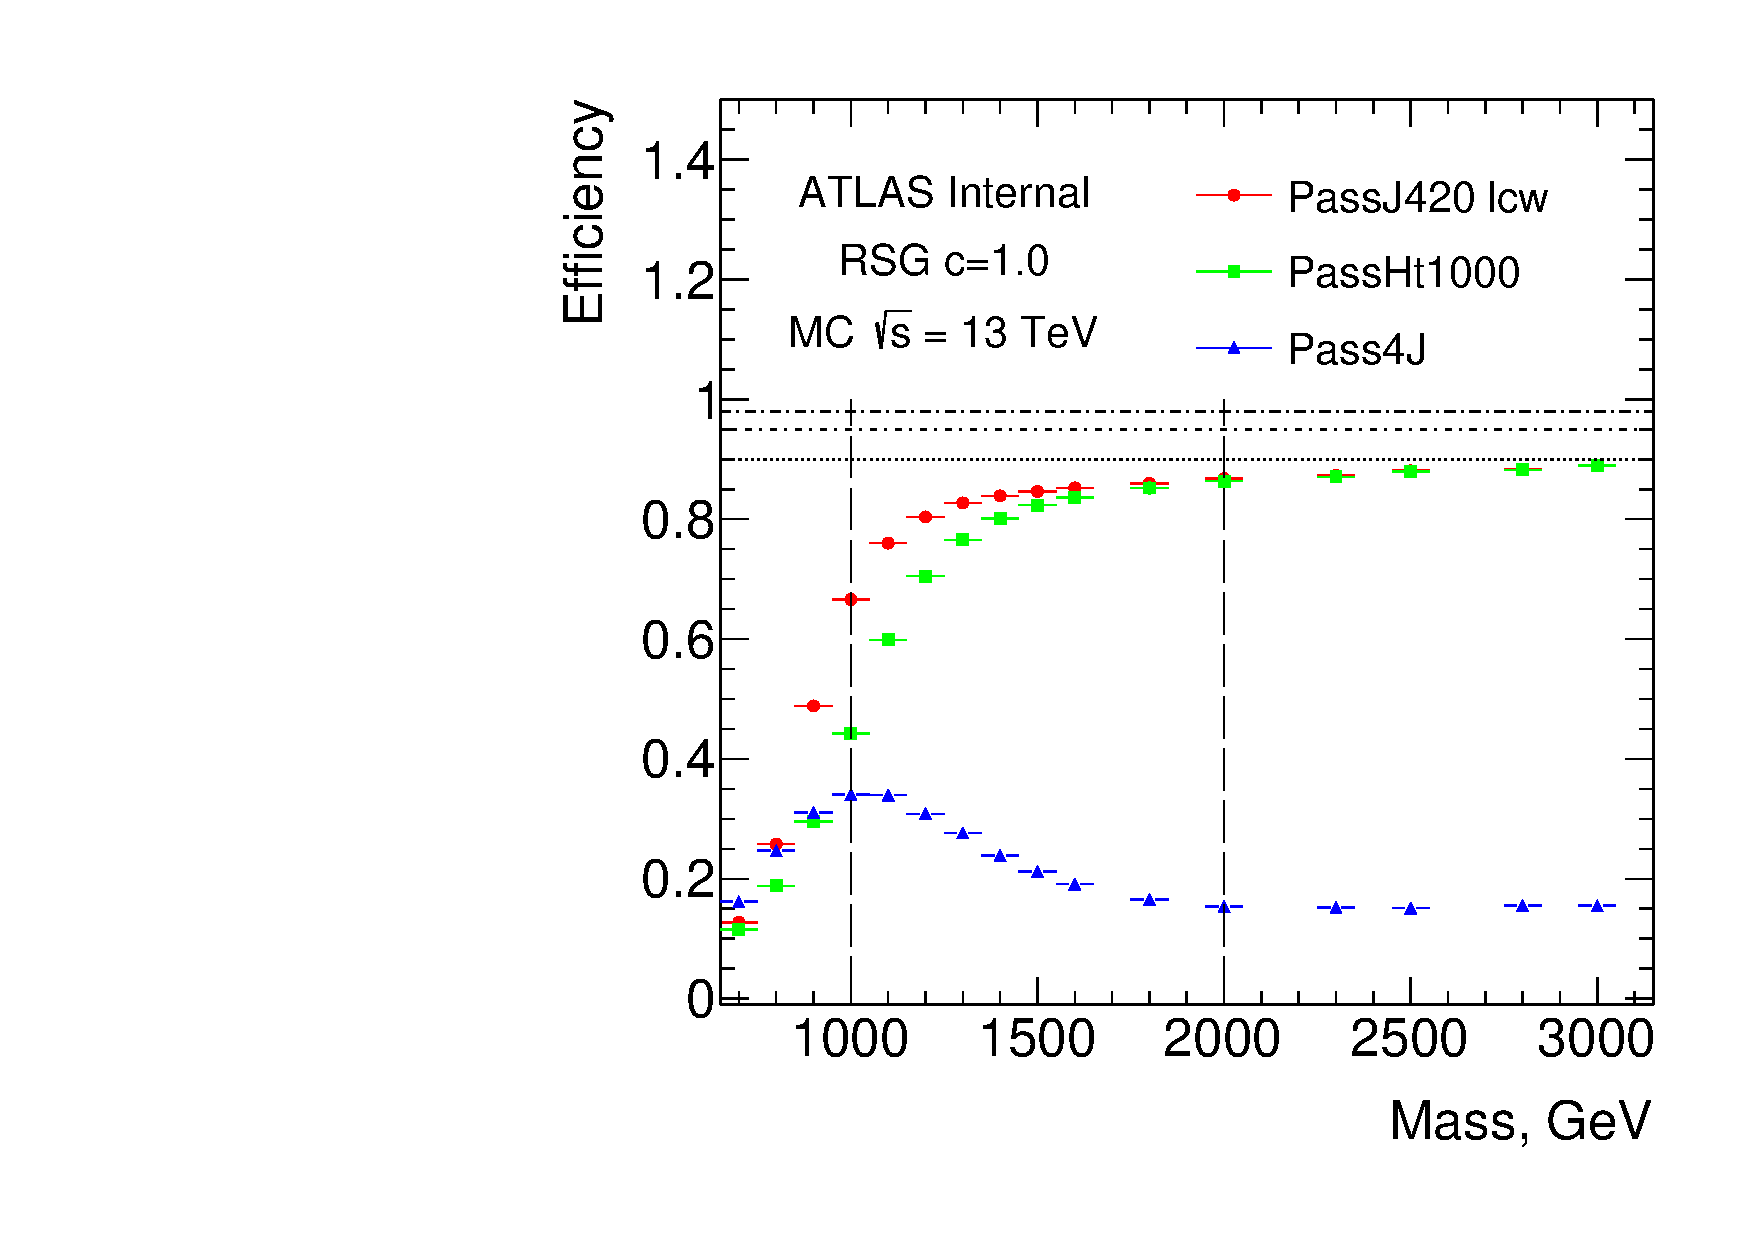
\includegraphics[width=0.45\textwidth,angle=-90]{figures/boosted/Trigger/app_trig_b77_Efficiency_PreSel.pdf}
  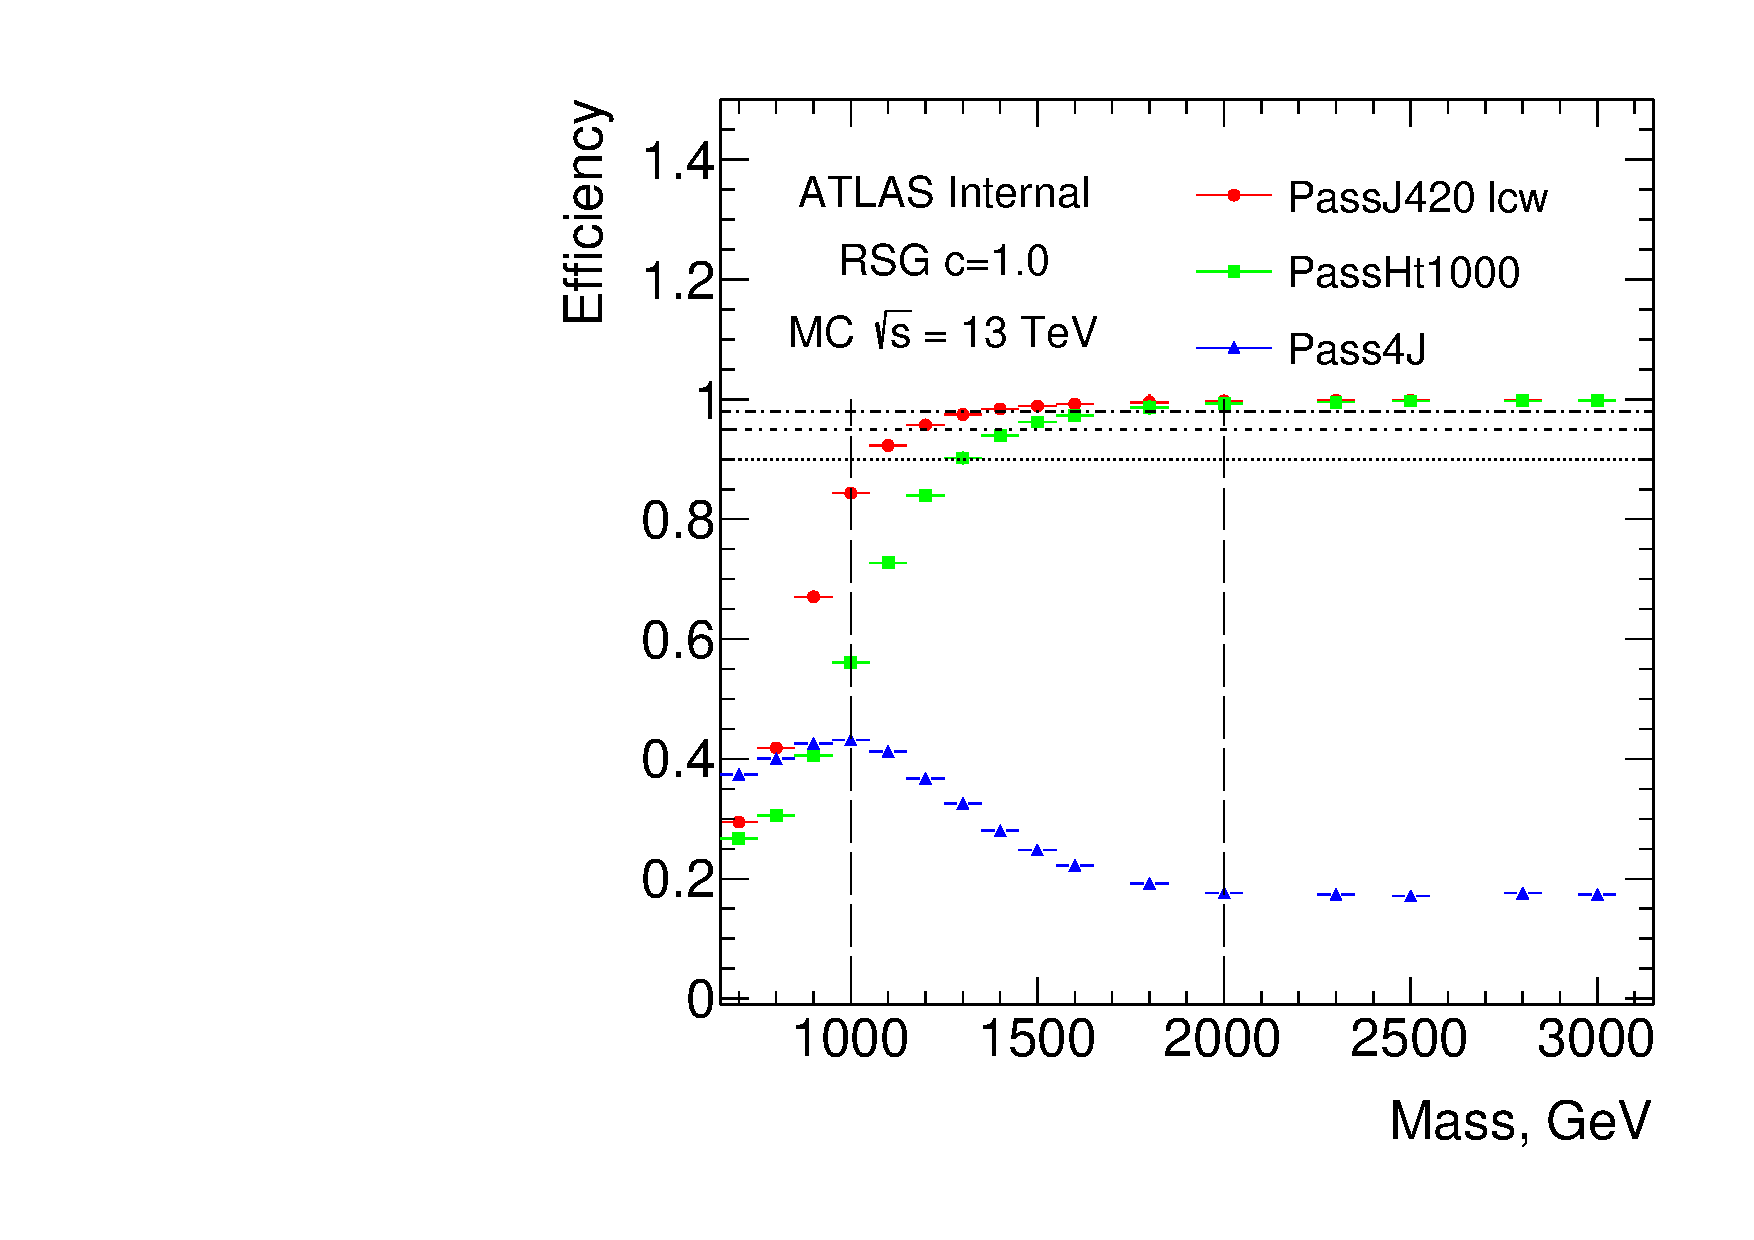
\includegraphics[width=0.45\textwidth,angle=-90]{figures/boosted/Trigger/app_trig_b77_Efficiency_All.pdf}
  %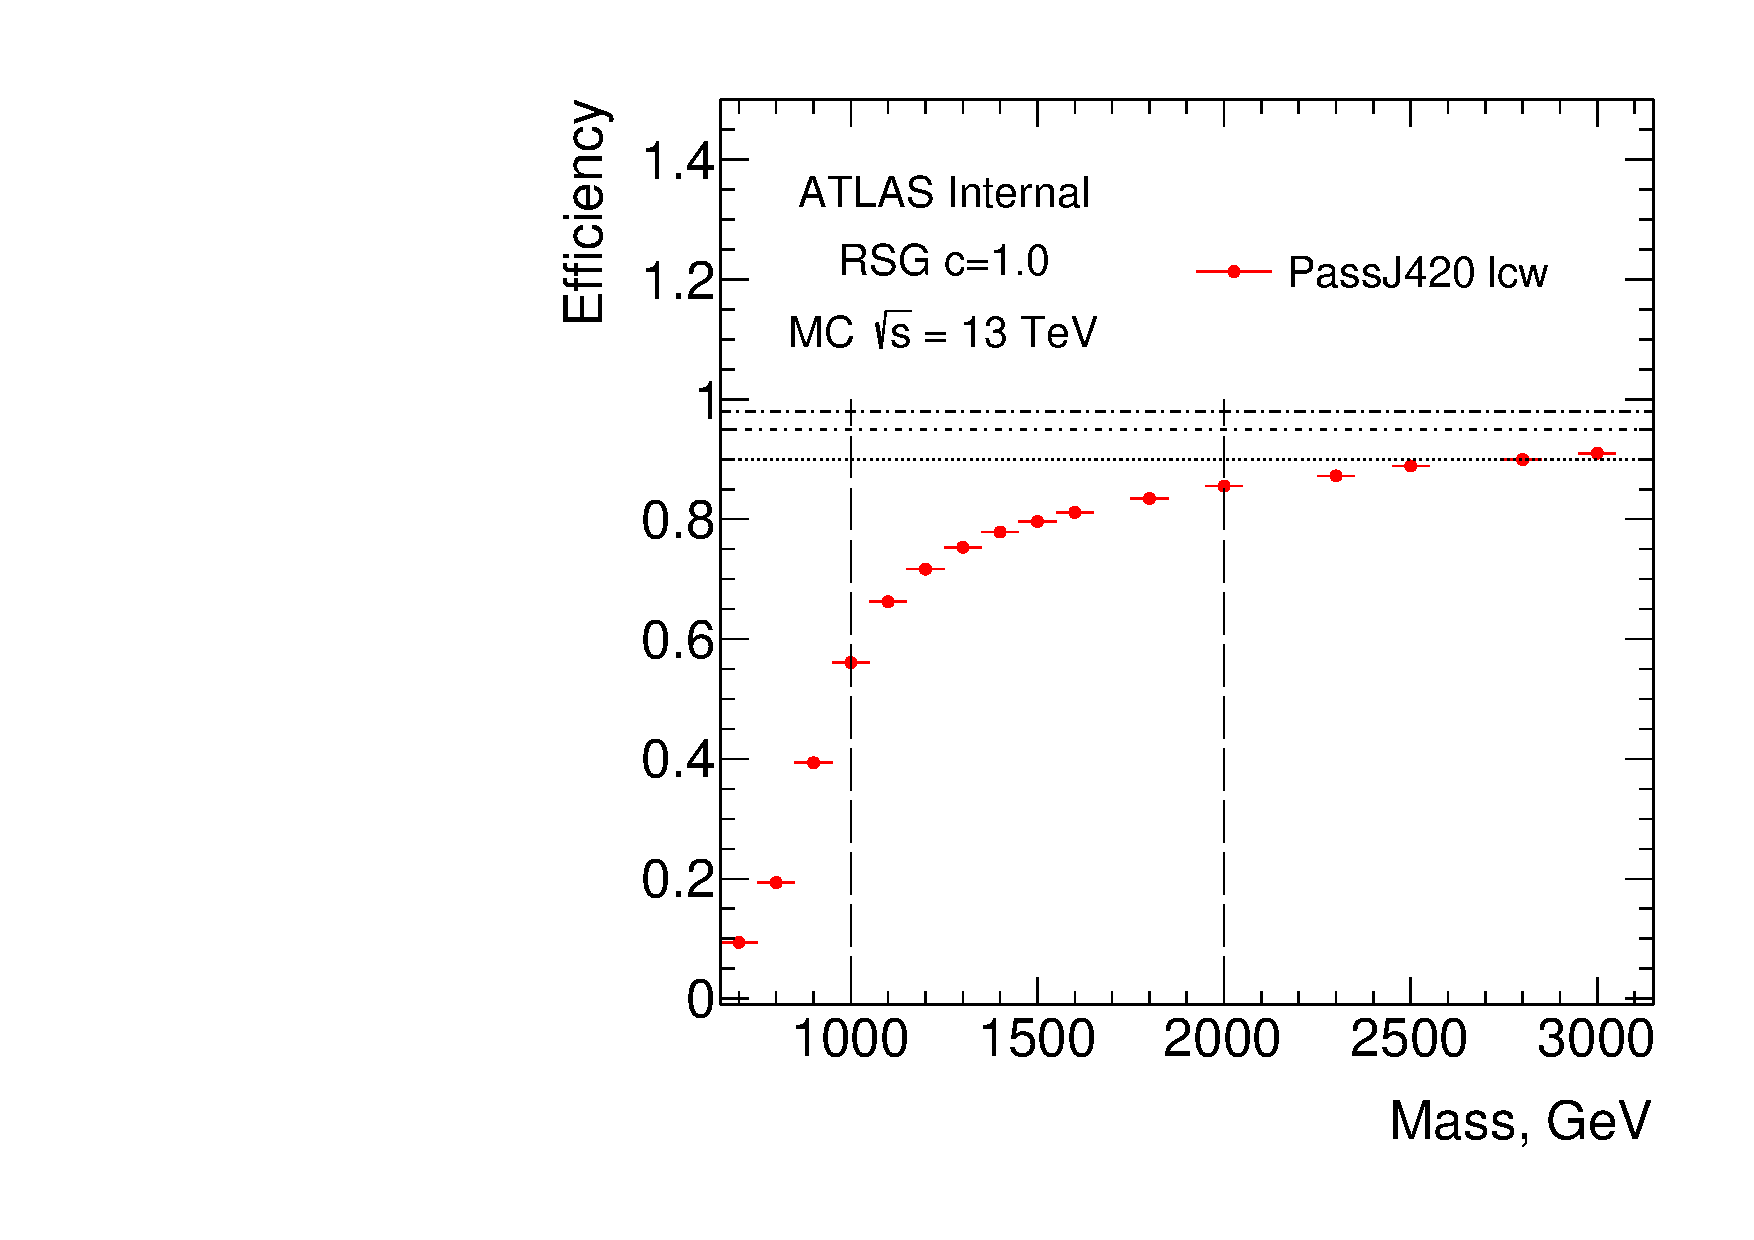
\includegraphics[width=0.45\textwidth,angle=-90]{figures/boosted/Trigger/trig_Moriond_Efficiency_PreSel.pdf}
  %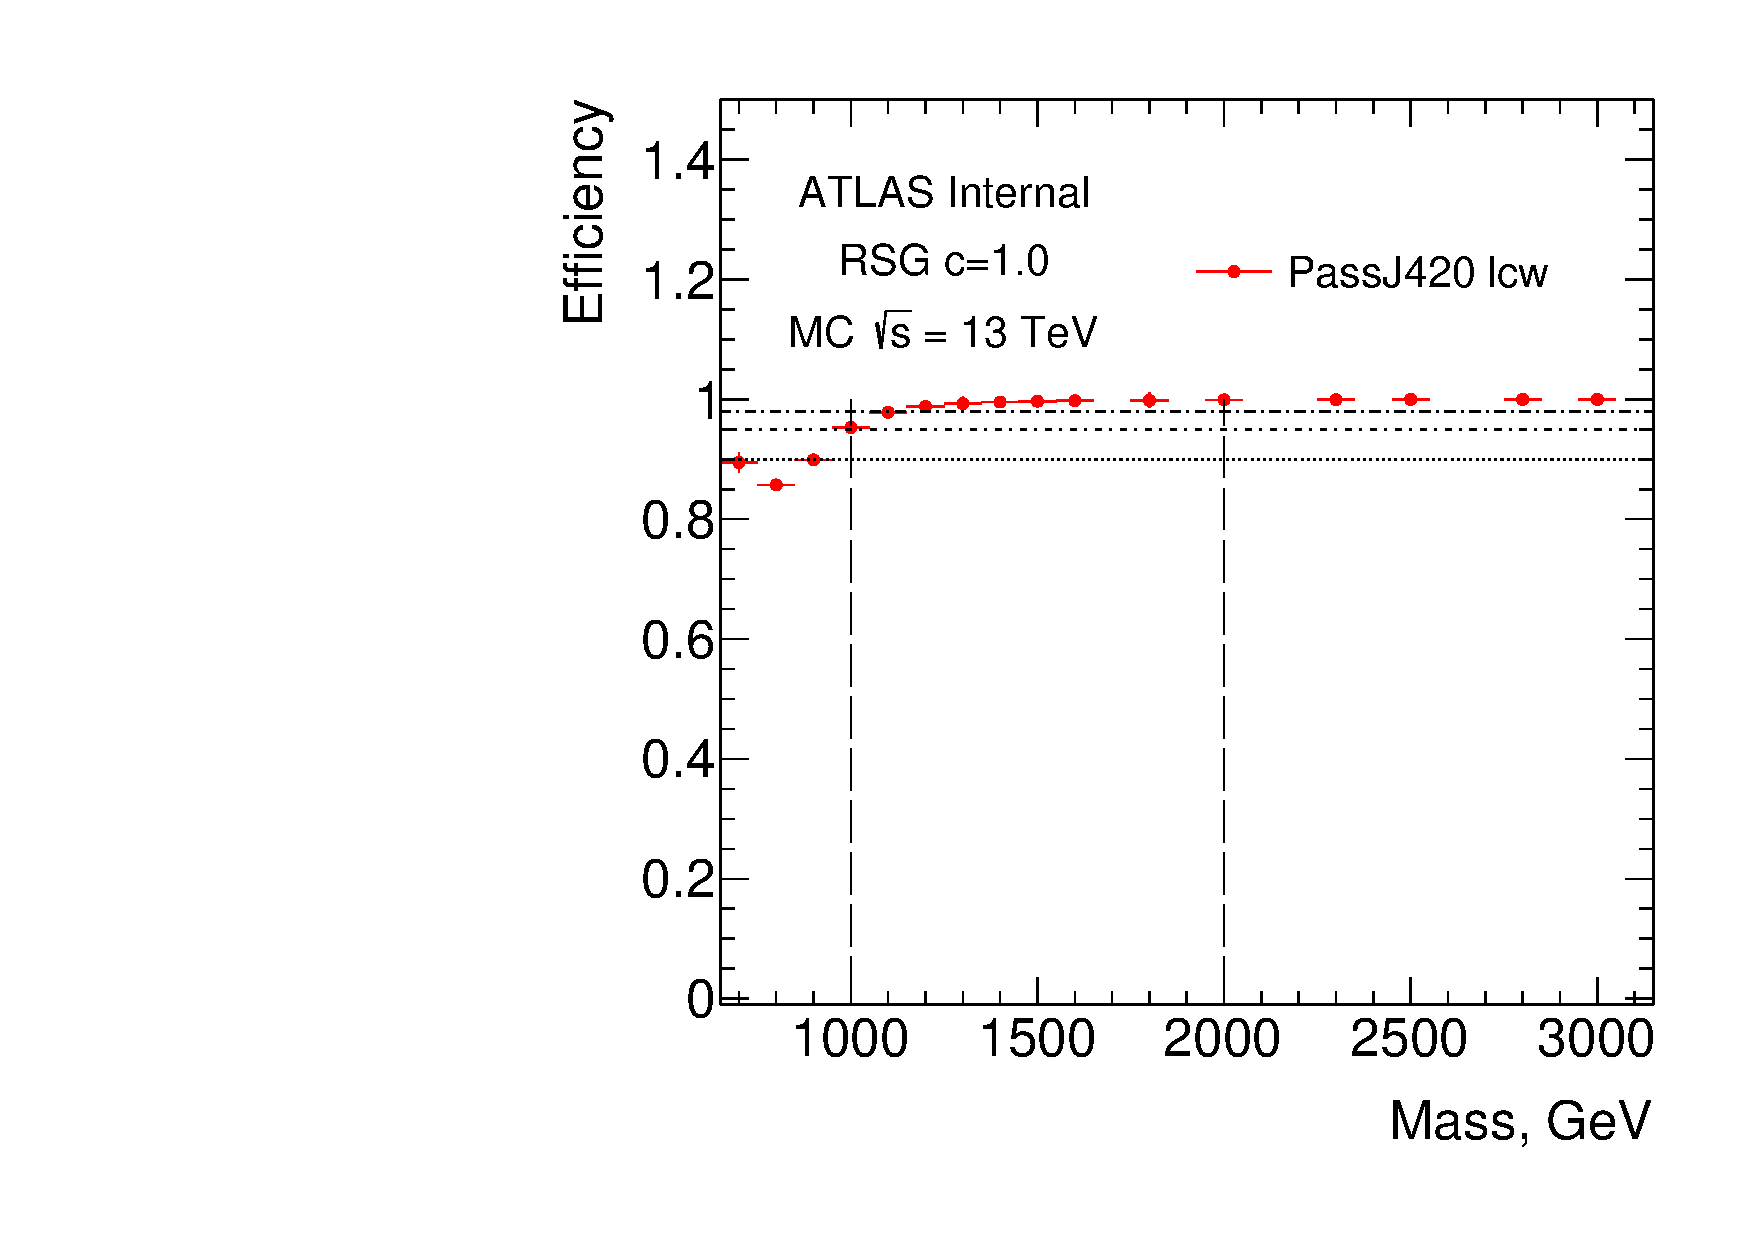
\includegraphics[width=0.45\textwidth,angle=-90]{figures/boosted/Trigger/trig_Moriond_Efficiency_All.pdf}
  \caption{Different trigger efficiencies as a function of the signal resonance mass with respect to all events with no selection (left) and with respect to events passing the two large-$R$ jets \pt > 400 \GeV and leading/subleading jet \pt > 250 \GeV (right). For 1.2 TeV signal, the trigger efficiency is about 95\%.}
  \label{fig:boosted-trigger-HLT}
\end{center}
\end{figure}

\label{evt-sel:trig}
\paragraph{}
The selected large-$R$ triggers are found to have $>98\%$ efficiency for signals with mass above 1200 \GeV, with the requirement that the event has two large-$R$ jets that satisfy the \pt requirements: leading jet \pt > 400 \GeV, and subleading jet leading jet \pt > 250 \GeV. The trigger turn-on curve in 2015 and 2016 data, as a function of leading jet \pt, is shown in Figure~\ref{fig:boosted-trigger-HLT-turnon}.
\begin{figure}[htbp!]
\begin{center}
  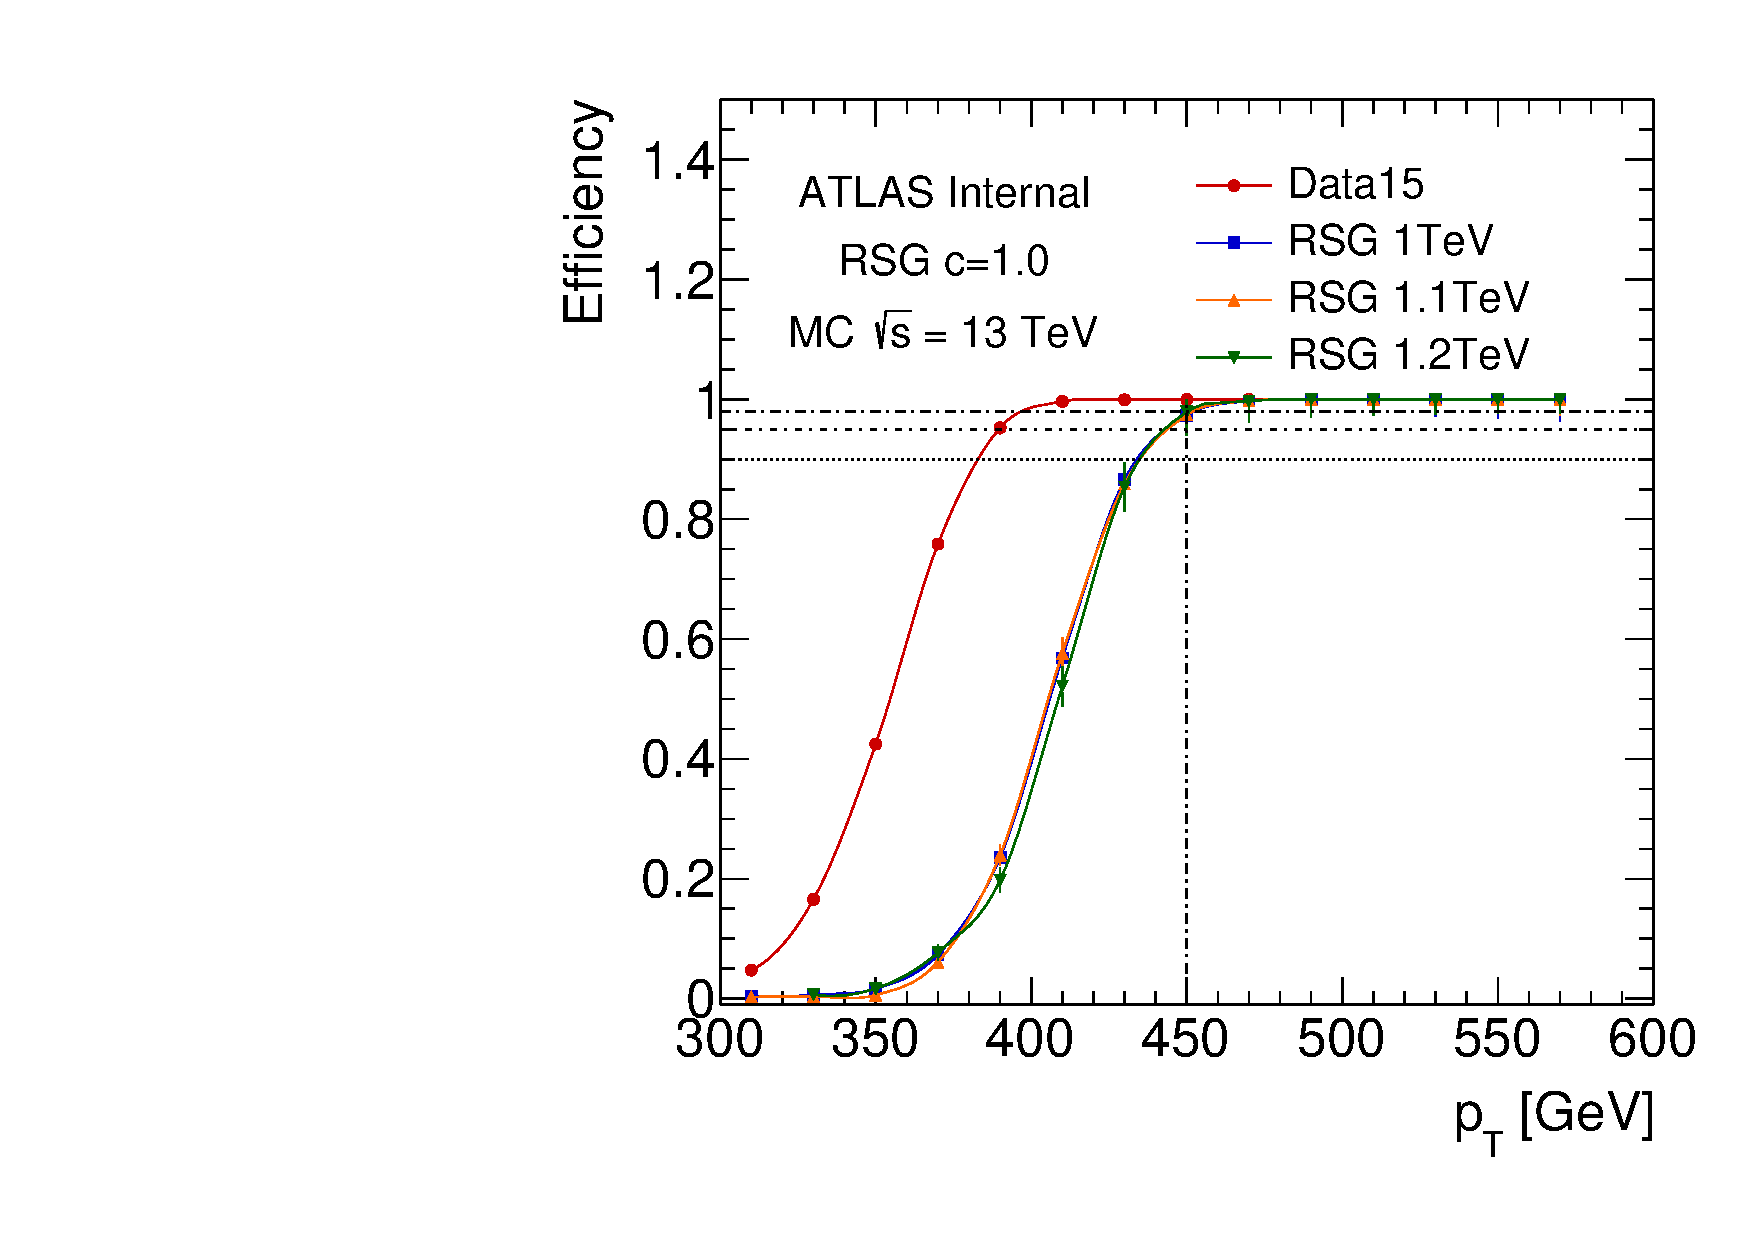
\includegraphics[width=0.45\textwidth,angle=-90]{figures/boosted/Trigger/trig_15_b77_pT_Efficiency.pdf}
  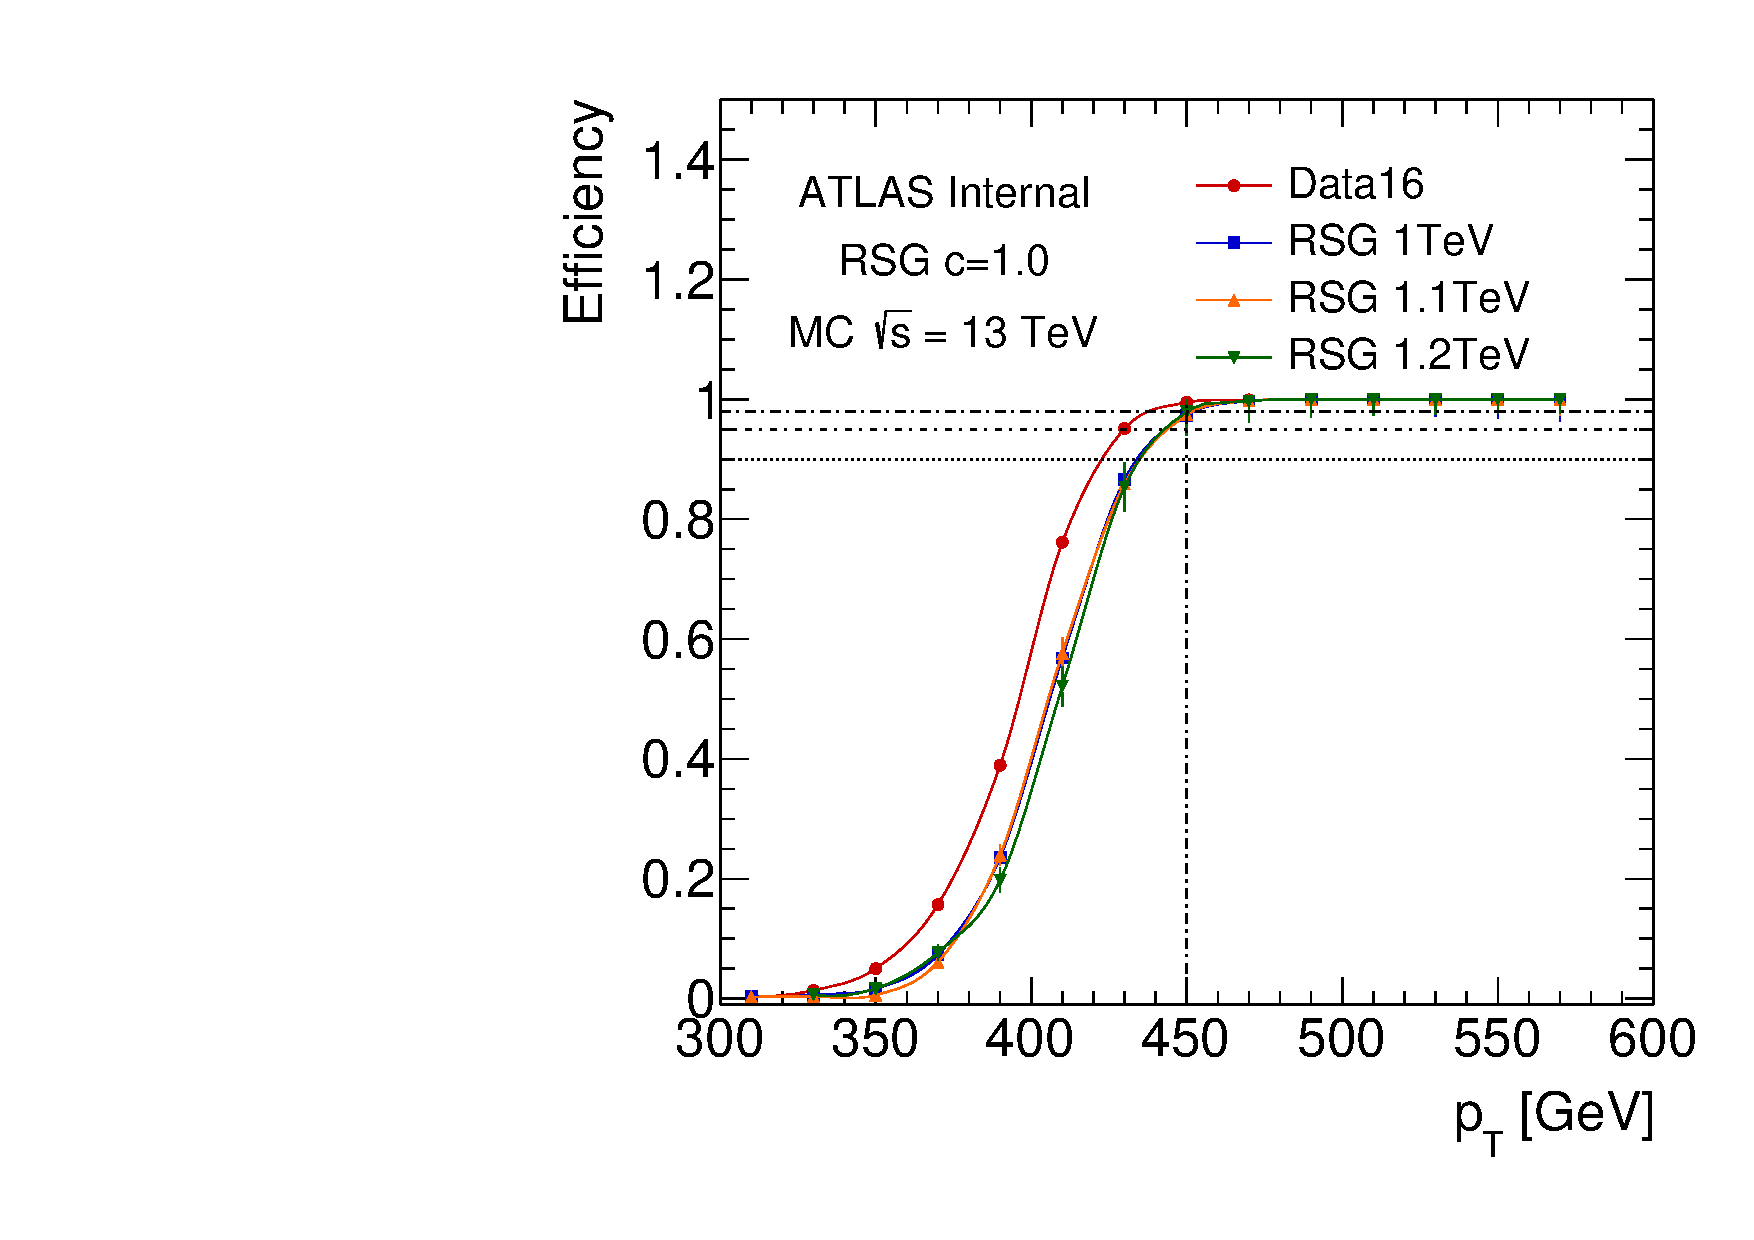
\includegraphics[width=0.45\textwidth,angle=-90]{figures/boosted/Trigger/trig_16_b77_pT_Efficiency.pdf}
  \caption{Large-$R$ jet trigger efficiencies, defined as the fraction of events fired trigger with a given leading large-$R$ jet \pt, measured in 2015 Data (\texttt{HLT\_j360\_a10\_lcw}, left) and 2016 Data (\texttt{HLT\_j420\_a10\_lcw}, right) and MC.}
  \label{fig:boosted-trigger-HLT-turnon}
\end{center}
\end{figure}

%%%%%%%%%%%%%%%%%%%%%%%%%%%%%%%%%%%%%%%%%%%%%%%%%%%%%%%%%%%%%%%%%%%%%%%%%%%%%%%%%%%%%%%%%%
\section{Object Preselection}
\paragraph{}
The specific physics objects used in the boosted analysis are described in previous sections and reiterated in Table~\ref{tab:boosted-objects}.

\begin{table}[bhp]
\begin{center}
\begin{tabular}{c|c}
  object & technical name \\
  \hline
  large-$R$ calorimeter jets & AntiKt10LCTopoTrimmedPtFrac5SmallR20Jets \\
  small-$R$ track jets       & AntiKt2PV0TrackJets \\
  b-tagging                  & on track jets, MV2c10, 70$\%$ working point \\
\end{tabular}
\caption{Physics objects and their technical names in the boosted analysis.} %%%
\label{tab:boosted-objects}
\end{center}
\end{table}

\paragraph{}
In addition to cleaning and trigger requirements, each event must have at least two high momentum large-$R$ jets, and each of these can have at least one ghost associated track jets for $b$-tagging. The large-$R$ jets are required to have \pt > 250 \GeV , $|\eta| < 2$,  and mass > 50 \GeV, while the leading \pt large-$R$ jet is also required to have \pt $> 450$ \GeV to be above the trigger threshold. The leading and sub-leading large-$R$ jets are considered the Higgs candidates. The track jets are required to have \pt $> 10 $ \GeV , $|\eta| < 2.5$ and at least two tracks associated with it.

\paragraph{}
A further muon correction accounts for energy loss due to leptonic $b$-hadron decays with a muon in the final state. The muon-in-jet corrections are applied only after the fiducial large-$R$ jet requirements on \pt and $\eta$. Combined muons with \pt > 4 \GeV, $|\eta| < 2.5$, and passing at least the medium MCP quality requirement are $\Delta R$ matched to the track jets within the large-$R$ jets. The muons are required have $\Delta R < 0.2$ with the $b$-tagged track jets. In case more than one muon is found within a track jet, only the muon with the smallest $\Delta R$ is considered. If two $b$-tagged track jets are found to have muons, both corrections are considered. The four-momenta of the matched muon is added to the large-$R$ jet four-momentum, with the muon calorimeter energy deposite substracted. This correction is only applied to the caloremeter mass portion of the combined mass. The muon-in-jet correction improves the large-R jet mass resolution by approximately 5\%, and Figure~\ref{fig:boosted-muons-signal} shows the impact of this correction on the 1 TeV signal sample.

\begin{figure*}
\begin{center}
  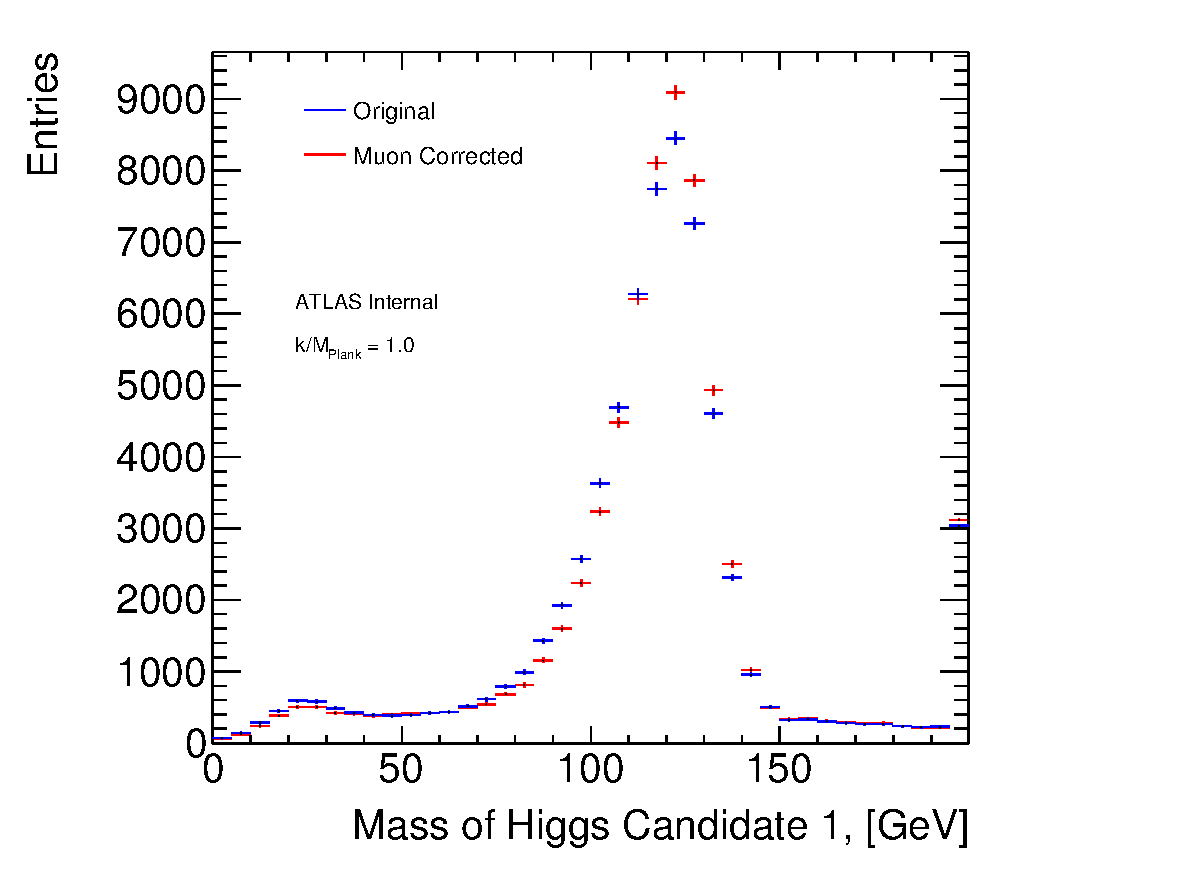
\includegraphics[width=0.48\textwidth]{figures/boosted/muons/h1_mass_dbl.pdf}
  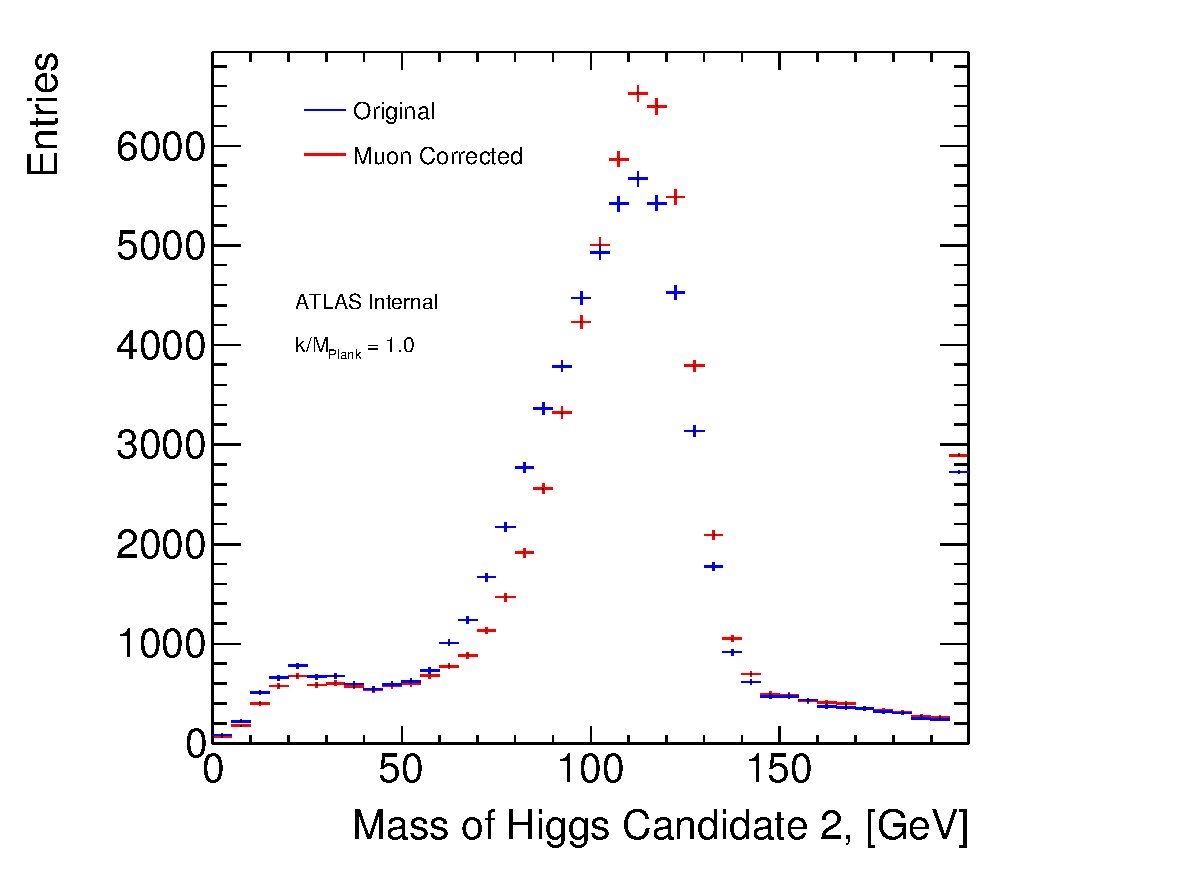
\includegraphics[width=0.48\textwidth]{figures/boosted/muons/h2_mass_dbl.pdf}
  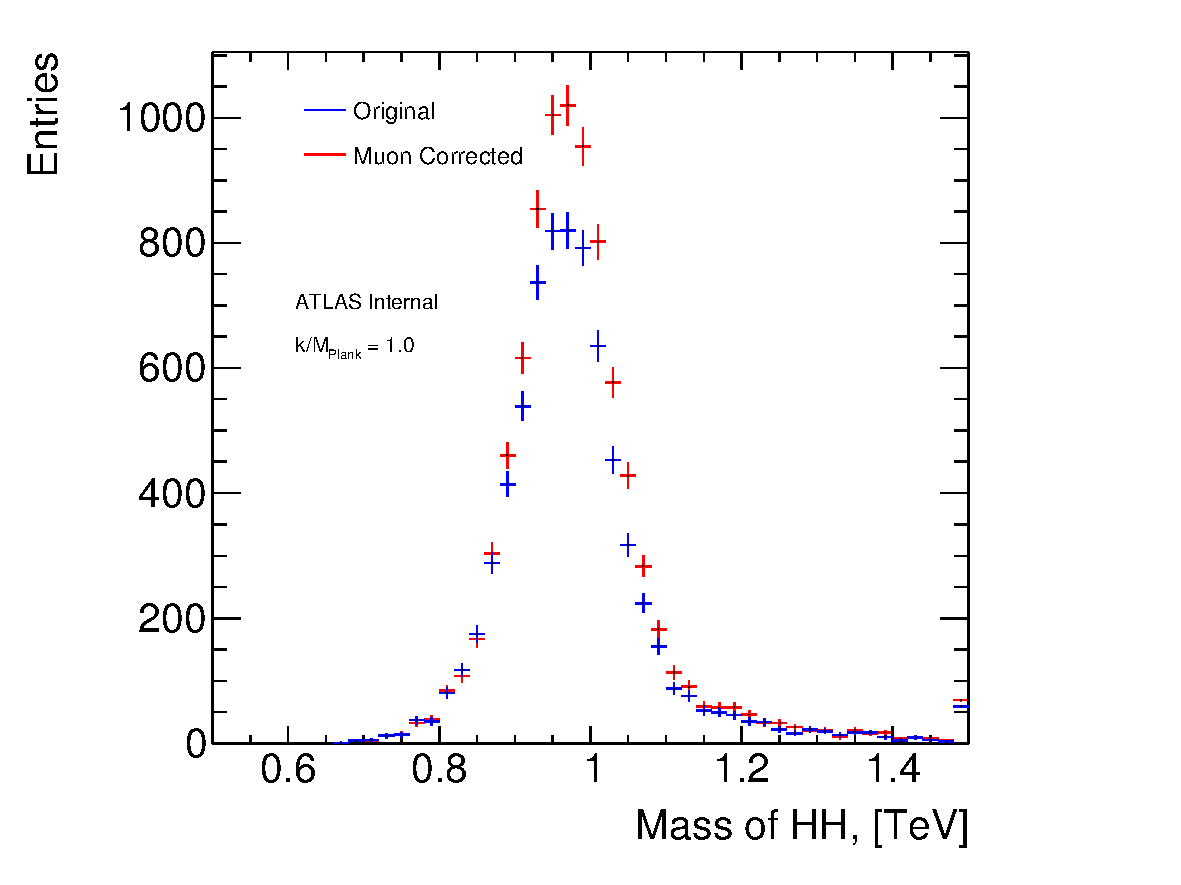
\includegraphics[width=0.48\textwidth]{figures/boosted/muons/hh_mass_dbl.pdf}
  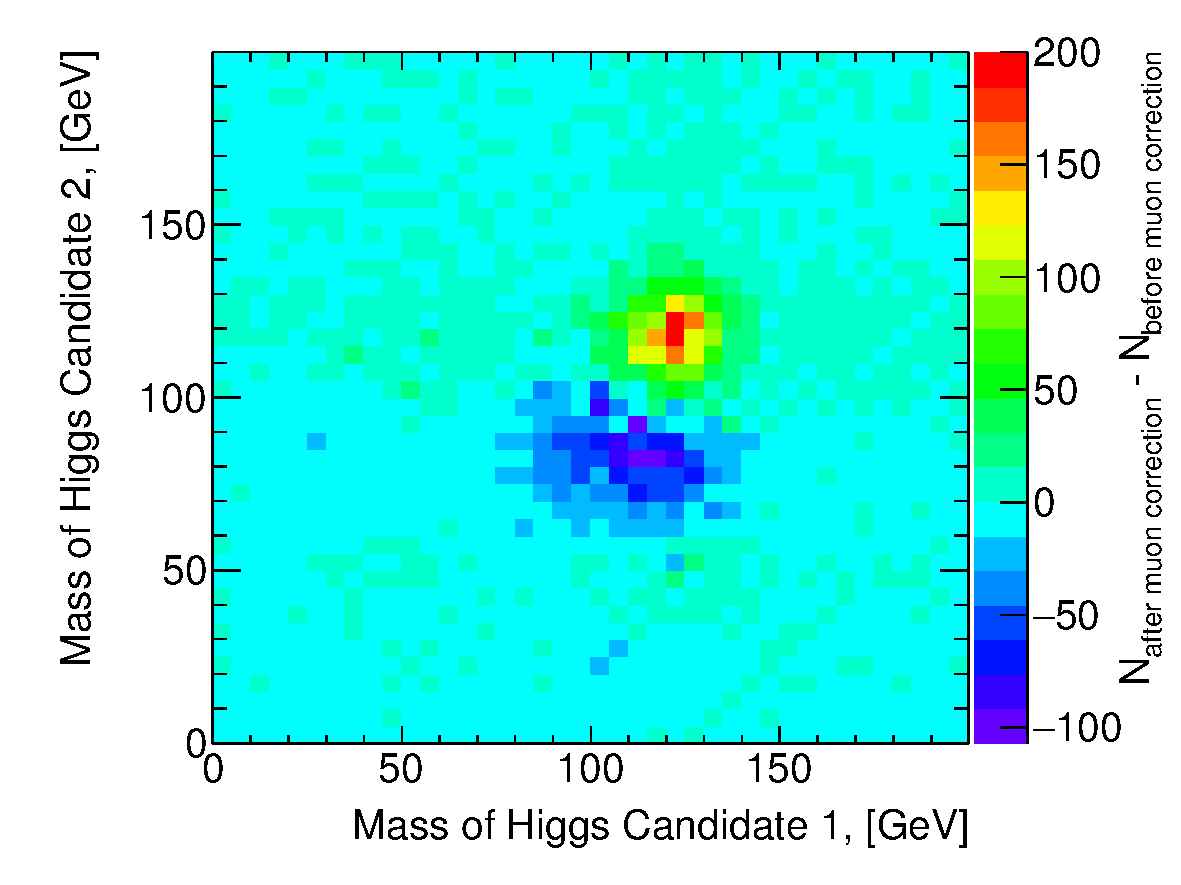
\includegraphics[width=0.48\textwidth]{figures/boosted/muons/h12_corr_mass.pdf}
  \caption{Kinematics of 1 TeV signal before and after muon-in-jet corrections. The reconstructed Higgs masses (top row, left for leading large-$R$ jet, right for subleading large-$R$ jet) are closer to 125 \GeV after the correction, which improves the signal efficiency for the signal region selection by $\sim\!10\%$ (bottom row, left for $m_{JJ}$, right for event distribution differences on the leading-subleading large-$R$ jet mass plane.).}
  \label{fig:boosted-muons-signal}
\end{center}
\end{figure*}

\paragraph{}
Finally, the Higgs candidates (large-$R$ jets) are also required to have $|\Delta\eta| = |\eta_{\text{leadJ}} -\eta_{\text{sublJ}} |< 1.7$. This is because signals are produced mostly through s-channel, while the multijet events could also be produced through t-channels or u-channel. Figure ~\ref{fig:app-check-deta} shows the distribution for signal sample and data inclusive $b$-tag region $\Delta \eta_{JJ}$ distribution.

\begin{figure*}
\begin{center}
  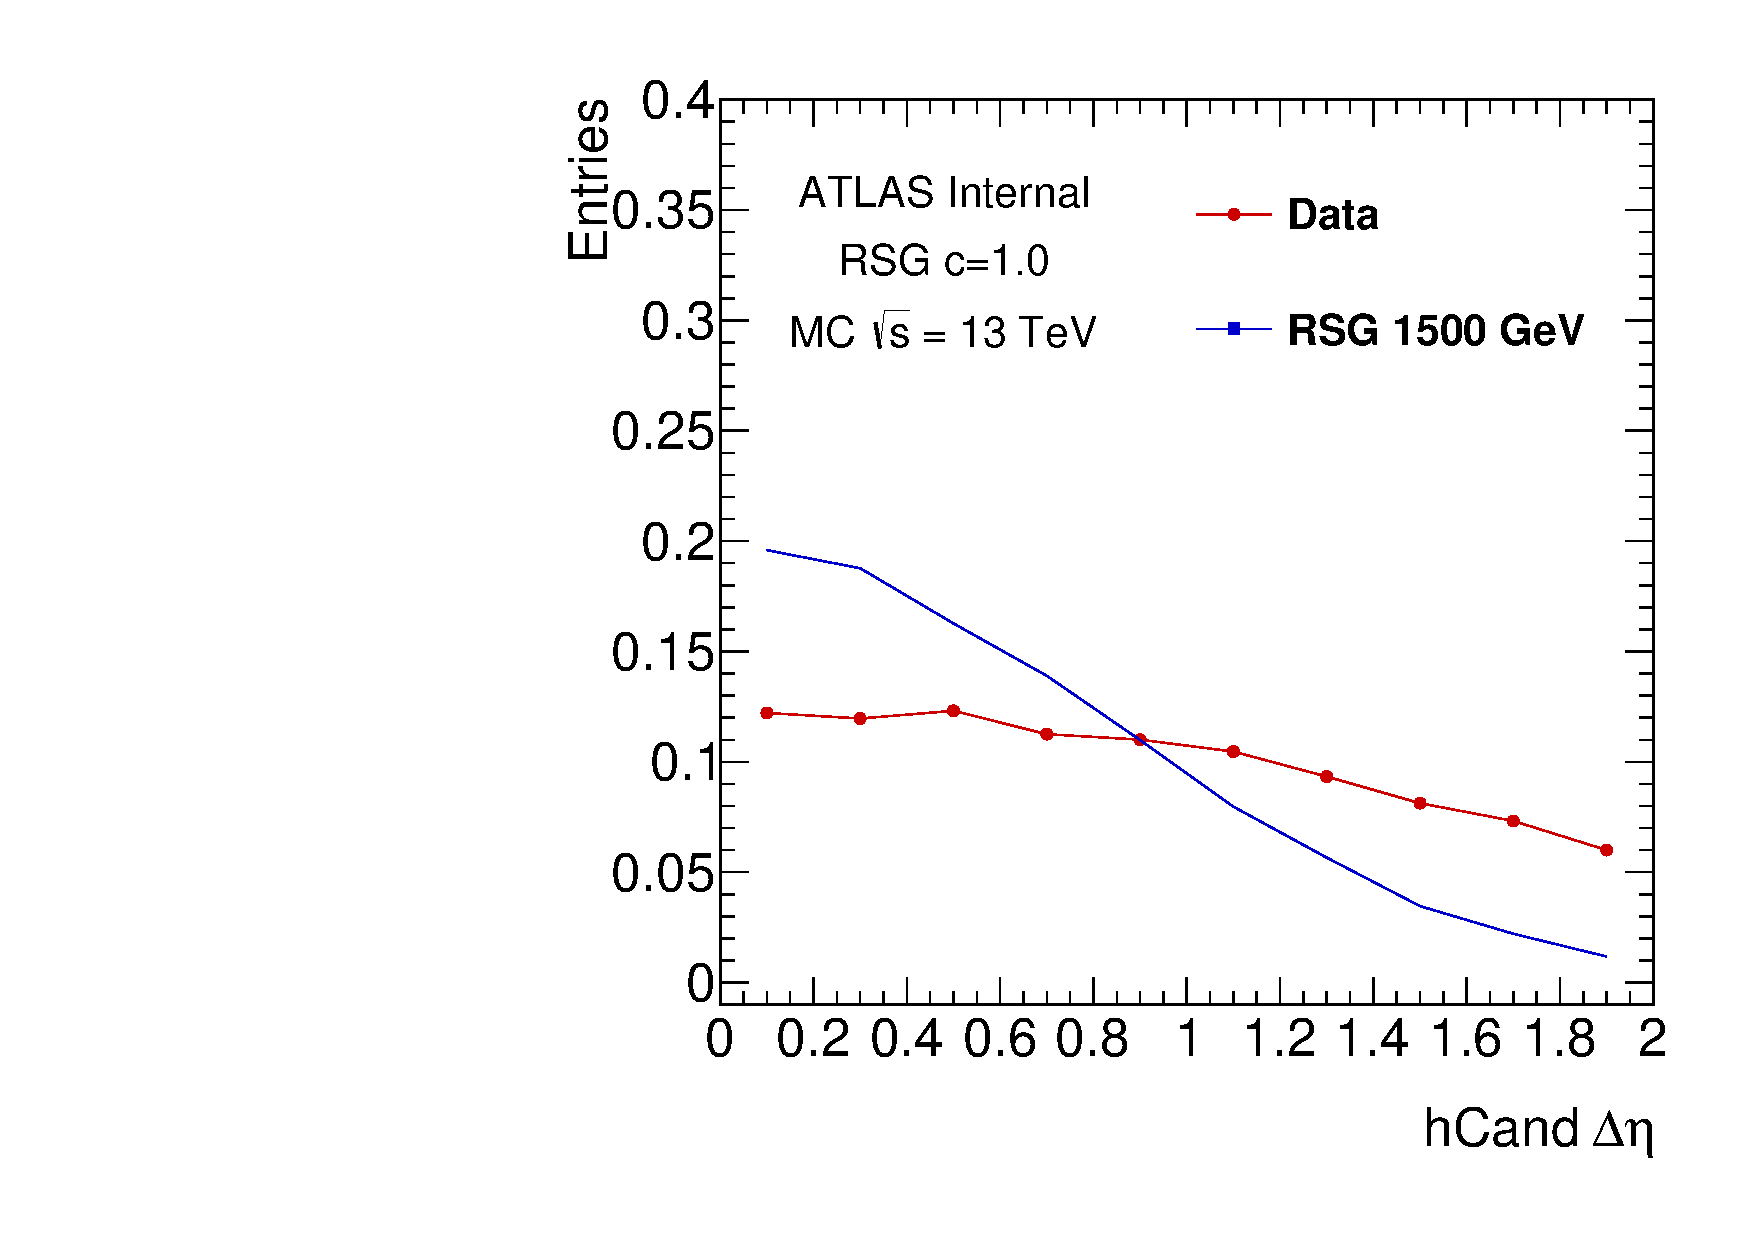
\includegraphics[width=0.45\textwidth,angle=-90]{figures/boosted/Other/AllTag_Signal_hCandDeta_F_c10-cb-no-deta-cut_truth_0.pdf}
  \caption{ After large-$R$ jet requirements, normalized $\Delta \eta_{JJ}$ distribution in signal MC and data, where the data consists of mostly multijet events (> 90$\%$). The QCD multijet tends to be more flat in $\Delta \eta_{JJ}$ distribution.}
\label{fig:app-check-deta}
\end{center}
\end{figure*}


%%%%%%%%%%%%%%%%%%%%%%%%%%%%%%%%%%%%%%%%%%%%%%%%%%%%%%%%%%%%%%%%%%%%%%%%%%%%%%%%%%%%%%%%%%
\section{Resolved Selection and Resolved Veto}
\label{sec:resollvedveto}
\paragraph{}
For resolved analysis, four jets with the highest $b$-tagging score are paired to construct two Higgs boson candidates. Pairings of jets into Higgs boson candidates are only accepted if they satisfy the following requirements, where \mfourj is expressed in \GeV:
if \mfourj  < 1250\,\GeV:
\begin{equation}
\frac{360\,\GeV}{\mfourj} - 0.5 < \DR_{jj}^{lead} < \frac{655\,\GeV}{\mfourj} + 0.475;
\frac{235\,\GeV}{\mfourj} < \DR_{jj}^{subl}  < \frac{875\,\GeV}{\mfourj} + 0.33
\end{equation}
if \mfourj  > 1250\,\GeV:
\begin{equation}
0< \DR_{jj}^{lead} < 1; 0 < \DR_{jj}^{subl} < 1
\end{equation}
In these expressions, $\DR_{jj, \mathrm{lead}}$ is the angular distance between jets in the leading Higgs boson candidate and $\DR_{jj, \mathrm{subl}}$ for the sub-leading candidate. The leading Higgs boson candidate is defined to be the candidate with the highest scalar sum of jet \pt. This requirement efficiently rejects jet-pairings where one of the $b$-tagged jets is not consistent with that originating from a Higgs boson decay. The specific cut values in this and the following requirements were chosen to maximize the sensitivity to the signal.

\paragraph{}
Events that have multiple Higgs boson candidates satisfying these requirements %(which happens often when $\mfourj < 500\,\GeV$),
necessitate an algorithm to choose the correct pairs. In the absence of energy loss through semi-leptonic decays, the optimal choice would be the combination most consistent with the decays of two particles of equal mass. (In principle, the masses should be that of the Higgs boson but explicitly requiring this does not significantly increase signal efficiency, while it sculpts the background Higgs boson candidate mass distributions to look like those of the signal, reducing the signal vs background discrimination in these variables.)

\paragraph{}
To account for energy loss, the requirement of equal masses is modified. The distance, \Dhh, of the pairing's leading and subleading Higgs boson candidate masses, $\left(\leadm, \sublm\right)$ from the line connecting $\left(0\,\GeV, 0\,\GeV\right)$ and $\left(120\,\GeV, 110\,\GeV\right)$ is computed, and the pairing with the smallest value of \Dhh is chosen. The values of 120\,\GeV\, and 110\,\GeV\, are chosen because they correspond to the median values of the narrowest intervals that contain 90\% of the signal in simulations.%the centre of the signal region in \leadm and \sublm respectively,
\Dhh can be expressed as follows:
\begin{equation}
D_{hh} = \frac{\left|\leadm - \frac{120}{110}\sublm\right|}{\sqrt{1+\left(\frac{110}{120}\right)^{2}}}.
\end{equation}

\paragraph{}
The resolved analysis searches for resonances with a wide range of masses, 260\,\GeV < \mhh < 1400\,\GeV, as well as non-resonant signals. Event selection criteria that vary as a function of the reconstructed di-Higgs-boson mass are used to reject background and hence enhance the analysis sensitivity across this range. Mass-dependent requirements are made on the leading Higgs boson candidate \pt, and the sub-leading Higgs boson \pt,:
\begin{equation}
p_T^{lead} > 0.5\mfourj - 105\,\GeV, \quad
p_T^{subl} > 0.33\mfourj - 75\,\GeV
\end{equation}
where \mfourj is again expressed in \GeV.

\paragraph{}
\begin{equation}
\dEta < 1.1 \mathrm{if}\ \mfourj < 850\,\GeV , \quad
\dEta < 2\times10^{-3} \mfourj - 0.6 \mathrm{if}\ \mfourj > 850\,\GeV
\end{equation}
A further (\mfourj-independent) requirement is placed on the pseudorapidity difference between the two Higgs boson candidates, $\dEta < 1.5$, which rejects multijet events.

\paragraph{}
A requirement on the Higgs boson candidates' masses is used to define the signal region:
\begin{equation}
\Xhh = \sqrt{\left(\frac{\mlead - 120\,\GeV}{0.1\mlead}\right)^2 + \left(\frac{\msubl - 110\,\GeV}{0.1\msubl}\right)^2} < 1.6,
\label{eqn:resolvedXhh}
\end{equation}
where the 0.1\mtwoj terms represent the widths of the leading and sub-leading Higgs boson candidate mass distributions, derived from simulation. The signal region is shown as the inner region of Figure~\ref{fig:resolvedRegions}.

\paragraph{}
In order to have statistical combination with the resolved analysis, events that pass the resolved signal region selections are vetoed. Specifically, for any event that has at least four AntiKt4EM jets passing \pt > 40 \GeV, $|\eta| < 2.5$, MV2c10 > 0.8244 (AntiKt4EM $70\%$ $b$-tagging working point), and if the event can make a higgs candidate through the Dhh minimization and passing through the resolved signal region Xhh cut, the event is not considered in the boosted selection. For more detail, please see the resolved signal region definition. For the impact on the boosted analysis, see Appendix ~\ref{sec:app-optimization-resveto}.

%%%%%%%%%%%%%%%%%%%%%%%%%%%%%%%%%%%%%%%%%%%%%%%%%%%%%%%%%%%%%%%%%%%%%%%%%%%%%%%%%%%%%%%%%%

\section{Signal Region}
%%\paragraph{}
After basic object selection, the signal region selection is defined by requiring multiple $b$-tags and jet masses which are consistent with the Higgs at 125 GeV. The presence of two \hbb decays in the final state naturally suggests requiring 4 track jets passing $b$-tagging requirements, and this is defined as the ``4$b$'' selection. However, since this requirement has an overall efficiency of roughly $\epsilon^4$, where $\epsilon$ is the efficiency of the tagger, a ``3$b$'' selection is also introduced to improve the signal efficiency, especially at high masses. In 4$b$ and 3$b$, one Higgs candidate can have at most two $b$-tagged trackjets, hence $\geq$ 3$b$-tagged trackjets cannot be in the same \largeR jet.At the highest resonance massed, the Lorentz boost of the Higgs boson can be large enough to collimate the daughter b-quarks below the distance scale resolvable by the track jets ($R=0.2$). Motivated by this, we introduce a third signal region --- which we denote by "two-tag-split" or simply  "$2bs$" --- in which exactly one $b$-tagged track jet is found in each Higgs candidate (plus an arbitrary number of track jets that do not pass the b-tag).

%%\paragraph{}
One major change since the 2015 analysis is the requirement on the number of track jets found in each \largeR\ jet.  In the past, each \largeR\ jet was required to contain at least two track jets in order to reduce and understand backgrounds.  However, above 2 TeV, this cut is inefficient for the signal, when the b-track-jets merge.  To recover this efficiency, we do not make any explicit requirement on the number of track jets in each \largeR\ jet.  Thus, an event with 3 $b$-tags must have at least 3 $b$-tagged track jets, but can have any number of additional un-tagged track jets. Similarly, an event with $2bs$ must have at least one b-tagged track jet in each of the \largeR\ jets. Again, the 70\% $b$-jet efficiency working point is used in the analysis.

%%\paragraph{}
To separate di-Higgs-boson decays from other multi-jet productions like QCD multi-jets and top, requirements on the leading and subleading large-$R$ jet masses are imposed. The signal region is defined using the expression:
\begin{equation}
\label{eq:boosted_XhhDef}
X_{hh} = \sqrt{\left(\frac{m^{\rm lead}_{\rm J} - \text{124 GeV}}{0.1 \left(m^{\rm lead}_{\rm J}\right)}\right)^2 + \left(\frac{m^{\rm subl}_{\rm J}- \text{115 GeV}}{0.1 \left(m^{\rm subl}_{\rm J}\right)}\right)^2}
%\begin{cases}
    %\sqrt{\left(\frac{m^{\rm lead}_{\rm J} - \text{124 GeV}}{0.085 \left(m^{\rm lead}_{\rm J}\right)}\right)^2 + \left(\frac{m^{\rm subl}_{\rm J}- \text{115 GeV}}{0.12 \left(m^{\rm subl}_{\rm J}\right)}\right)^2}, & \text{if } p_{T}^{\rm lead} < \text{900 GeV}\\
    %\sqrt{\left(\frac{m^{\rm lead}_{\rm J} - \text{124 GeV}}{0.085 \left(m^{\rm lead}_{\rm J}\right)}\right)^2 + \left(\frac{m^{\rm subl}_{\rm J}- \text{115 GeV}}{0.12 \left(m^{\rm subl}_{\rm J}\right)}\right)^2} - 0.4 (\frac{p_{T}^{\rm lead}}{\text{900 GeV}} - 1),              & \text{if } p_{T}^{\rm lead} \geq \text{900 GeV}
%\end{cases}
\end{equation}

%%\paragraph{}
The denominator of each term in the definition can be interpreted as a resolution on the reconstructed mass of $10\%$ for the leading and subleading jets, hence $X_{hh}$ can be interpreted as a $\chi^2$ compatibility with the $hh$ hypothesis. Similarly to the resolved analysis, these $\sigma \left(m_{\rm J}\right)$ are only a rough approximation to the true resolution, but the $X_{hh}$ requirement gives nearly optimal performance. The subleading jet mass value of 115\,GeV  is chosen after investigating the signal jet masses in MC and noticing that the subleading large-$R$ jet typically has a reconstructed mass which is biased downward. This is due to the ordering of the large-$R$ jets in $p_\text{T}$, which biases the sub-lead jet towards lower energy. The energy losses result from neutrinos in leptonic $b$ decays, cracks in the calorimeter, and other effects. The signal region requires $X_{hh} < 1.6$, same as the resolved analysis. 

%The denominator of each term in the definition can be interpreted as a resolution on the reconstructed mass of $8.5\%$ for the leading jet and $12\%$ for the subleading jet, hence $X_{hh}$ can be interpreted as a $\chi^2$ compatibility with the $hh$ hypothesis. Similarly to the resolved analysis, these $\sigma \left(m_{\rm J}\right)$ are only a rough approximation to the true resolution, but the $X_{hh}$ requirement gives nearly optimal performance. 
%The last substraction for high $p_\text{T}$ cases is because of the higher mass resolution of high mass signal samples. This effectively increases the size of $X_{hh}$ to 1.8 for a 3 TeV signal.

%%\paragraph{}
A similar circular variable can be defined in the two-dimensional mass plane, $R_{hh}$. The circular region $R_{hh}$ has the same central values as $X_{hh}$, but without resolution terms in the denominators and is defined as:
\begin{equation}
\label{eq:boosted_RhhDef}
R_{hh} = \sqrt{\left(m^{\rm lead}_{\rm J} - \text{124 GeV}\right)^2 + \left(m^{\rm subl}_{\rm J} - \text{115 GeV}\right)^2}
\end{equation}

%%\paragraph{}
The region defined by $1.6 < X_{hh}$ and $R_{hh} < 33$ will be used later in the definition of control regions, as discussed in Section~\ref{sec:boosted-qcd}. The cut value was optimized to allow for a reasonable sized sample (twice the statistics as the signal region) in the control region with kinematics similar to the signal region, whilst avoiding the large contributions of the $t\bar{t}$ sample when the large-$R$ jets have a mass near the top quark mass (i.e. with $m_J > 160$~\GeV).

%%\paragraph{}
Similarly, $R_{hh}^{\text{high}}$, the circular region that has the shifted central values up by 10 $GeV$ is defined using the variable:\begin{equation}
\label{eq:boosted_RhhhighDef}
R_{hh}^{\text{high}} = \sqrt{\left(m^{\rm lead}_{\rm J} - \text{134 GeV}\right)^2 + \left(m^{\rm subl}_{\rm J} - \text{125 GeV}\right)^2}
\end{equation}

%%\paragraph{}
In Run-1, and in the the 2015 analysis, the sideband was defined to be all events not in the signal or control regions. However, the kinematics of events with very large and very small large-R jet masses may not be the same as those within the signal region. Thus, to avoid biasing effects from extremely low mass or extremely high mass large-$R$ jets, the sideband region is also redesigned to be like the control region, but at $R_{hh} > 33$ and $R_{hh}^{\text{high}} < 58$. The shift upwards helps to capture enough $t\bar{t}$ events in the normalization estimates, as described in Section ~\ref{sec:ttbarnorm}. A similar sideband definition with an upper limit has been made for the resolved analysis.

%%\paragraph{}
The values of the $X_{hh}$ and $R_{hh}$ variables can be seen graphically in Figure~\ref{fig:boosted-regiondef-cartoons}.
\begin{figure}[htbp!]
\begin{center}
  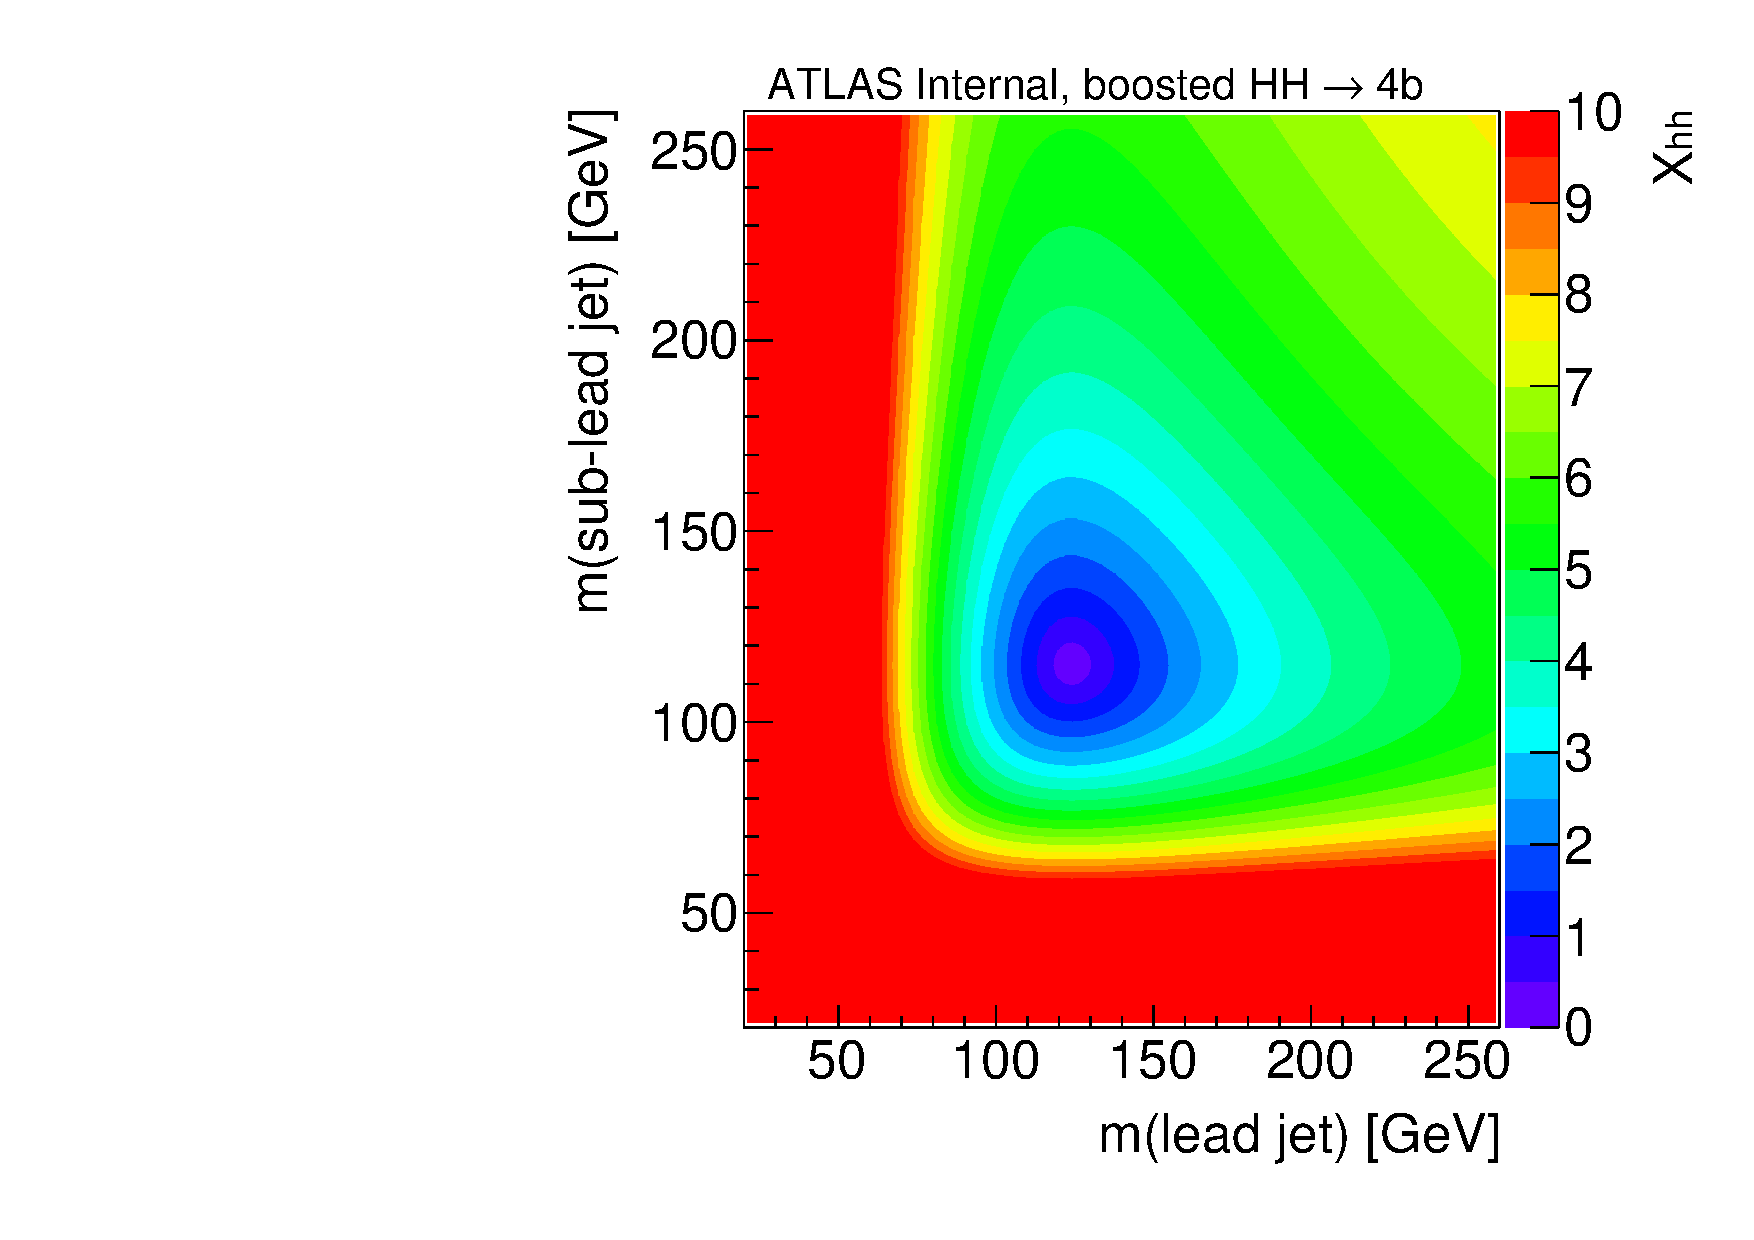
\includegraphics[width=0.48\textwidth,angle=-90]{figures/boosted/Other/cartoon-xhh.pdf}
  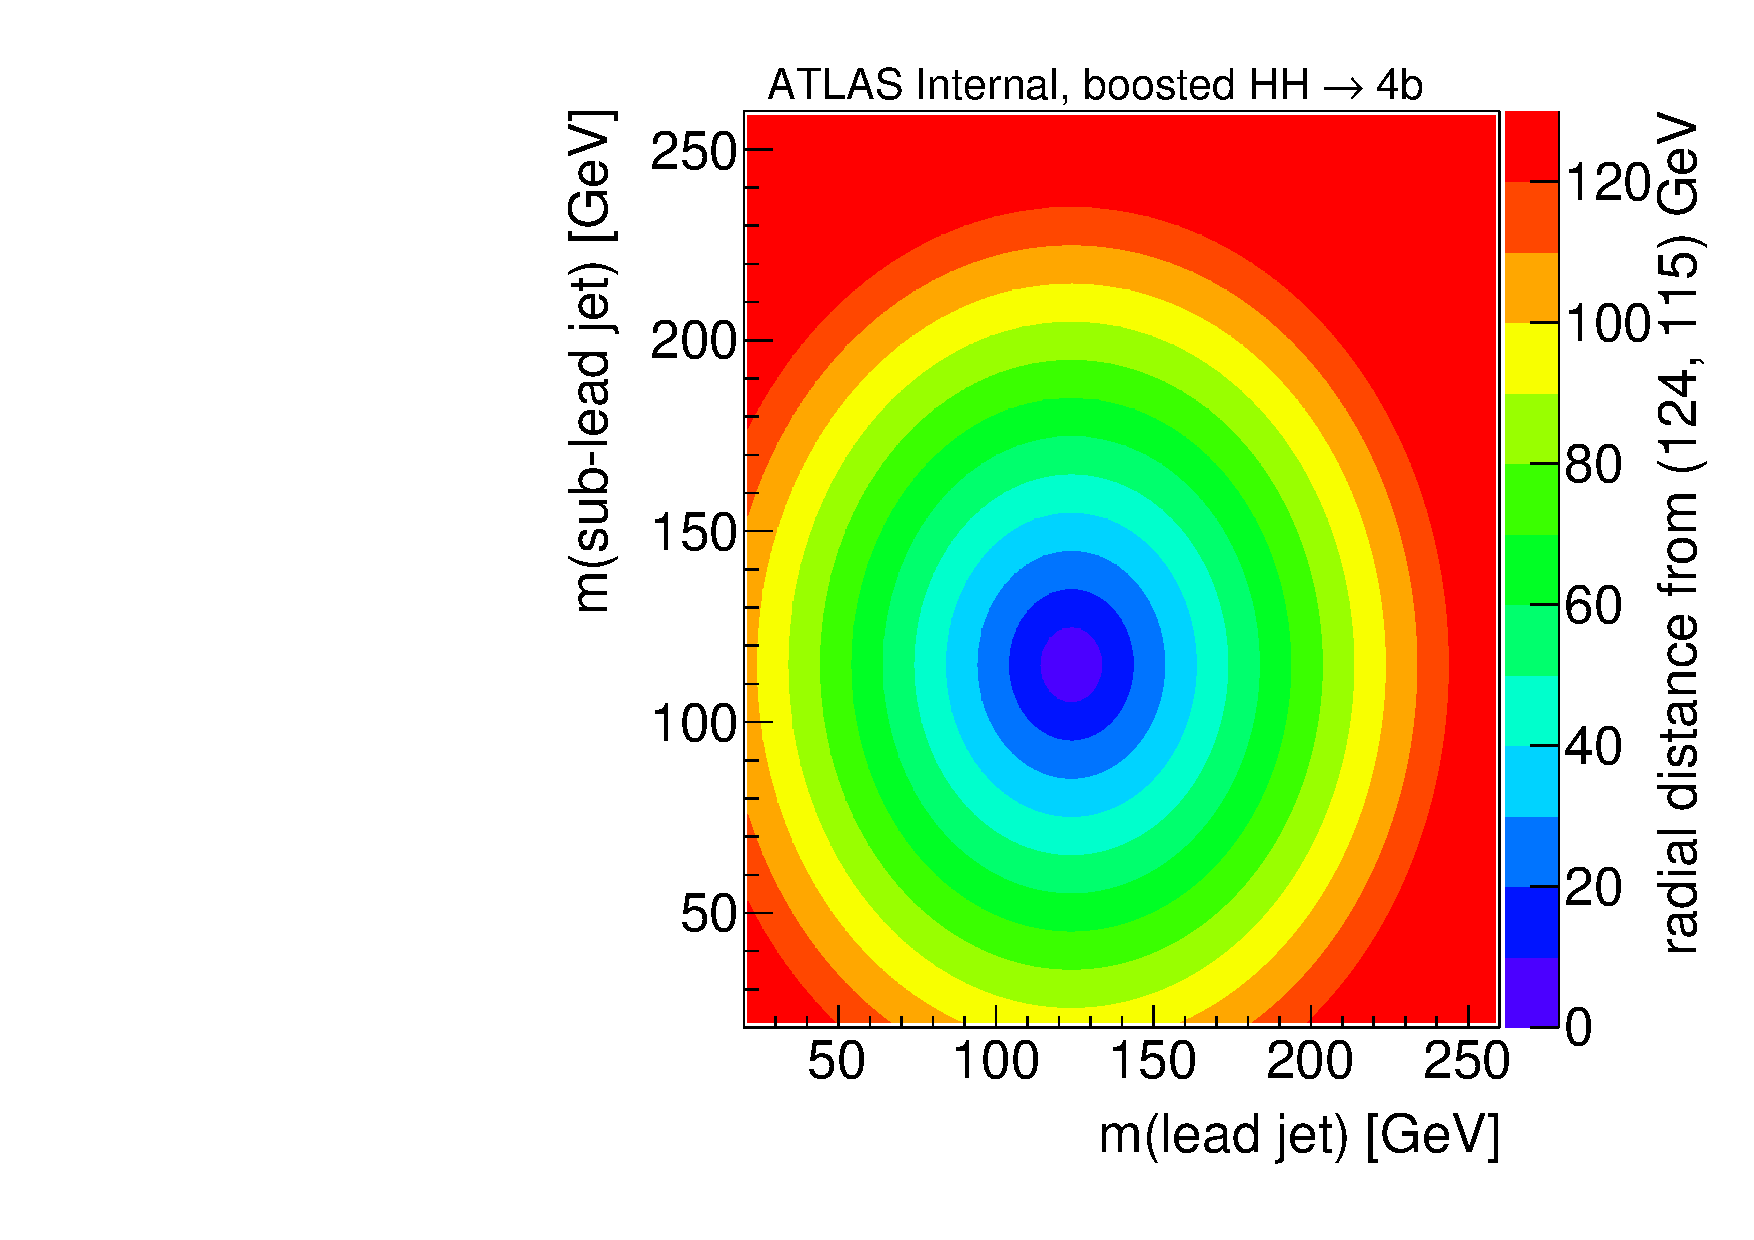
\includegraphics[width=0.48\textwidth,angle=-90]{figures/boosted/Other/cartoon-rhh.pdf}
  \caption{Values of the $X_{hh}$ and $R_{hh}$ variables, which are shapes in the two-dimensional plane of the large-R jet masses used to defined signal, control, and sideband regions. For both variables, a smaller value indicates the jets are closer to the Higgs mass. }
  \label{fig:boosted-regiondef-cartoons}
\end{center}
\end{figure}


\section{Signal efficiency}
\paragraph{}
Acceptance means purely geometric fiducial volume of the detector. Efficiency refers to purely detector effectivenss in finding objects. The final value in the study is Acceptance $\times$ Efficiency, where both effects are considered.

\paragraph{}
The boosted analysis covers multiple TeV of signal resonance masses, and the backgrounds fall steeply as a function of the reconstructed di-Higgs mass. Understanding how the signal efficiency trends with resonance mass can be helpful in gauging the natural limitations of very boosted objects. It can also indicate ways to improve sensitivity, as the resolved analysis has implemented with mass-dependent cuts, though the boosted analysis is currently not exploring this option.

%%\paragraph{}
The signal efficiency as a function of resonance mass is shown in Figure~\ref{fig:boosted-selection-efficiency}, both for the absolute signal efficiency and for the efficiency relative to the previous cut in the selection. Above a mass of $\sim\!1$ TeV, the reconstruction of high momentum large-$R$ jets with small $\Delta\eta$ is efficient. Across the mass range considered, the signal jet masses requirement ($X_\text{hh}$) and $b$-tagging requirements are $\mathcal{O}(20\%)$ efficient relative to the previous cuts. 

%%\paragraph{}
Above a mass of $\sim\!2$ TeV, the requirement of two track jets per large-$R$ jet becomes increasingly inefficient due to the merging of the track jets. This motivates introducing a selection without a requirement on the number of track jets, and to sort the signals based on the corresponding number of $b$-tagged track jets, as shown in Figure~\ref{fig:boosted-selection-signal-efficiency}. At high masses above 2.5 TeV, the 2$b$s region (where each large-$R$ jet has exactly one $b$-tagged track jet) significantly improves the sensitivity. In this figure, 2$b$ region is defined as a mutually exclusive region (where one large-$R$ jet has two $b$-tagged track jets, and the other one has no $b$-tagged track jet). The number of events in the control region and sideband region as a function of Resonance mass is shown in Figure~\ref{fig:boosted-selection-region-efficiency}. For 2$b$s, 3$b$ and 4$b$, each region has the number of events decrease from signal region to control region to sideband regions.

\begin{figure*}
\begin{center}
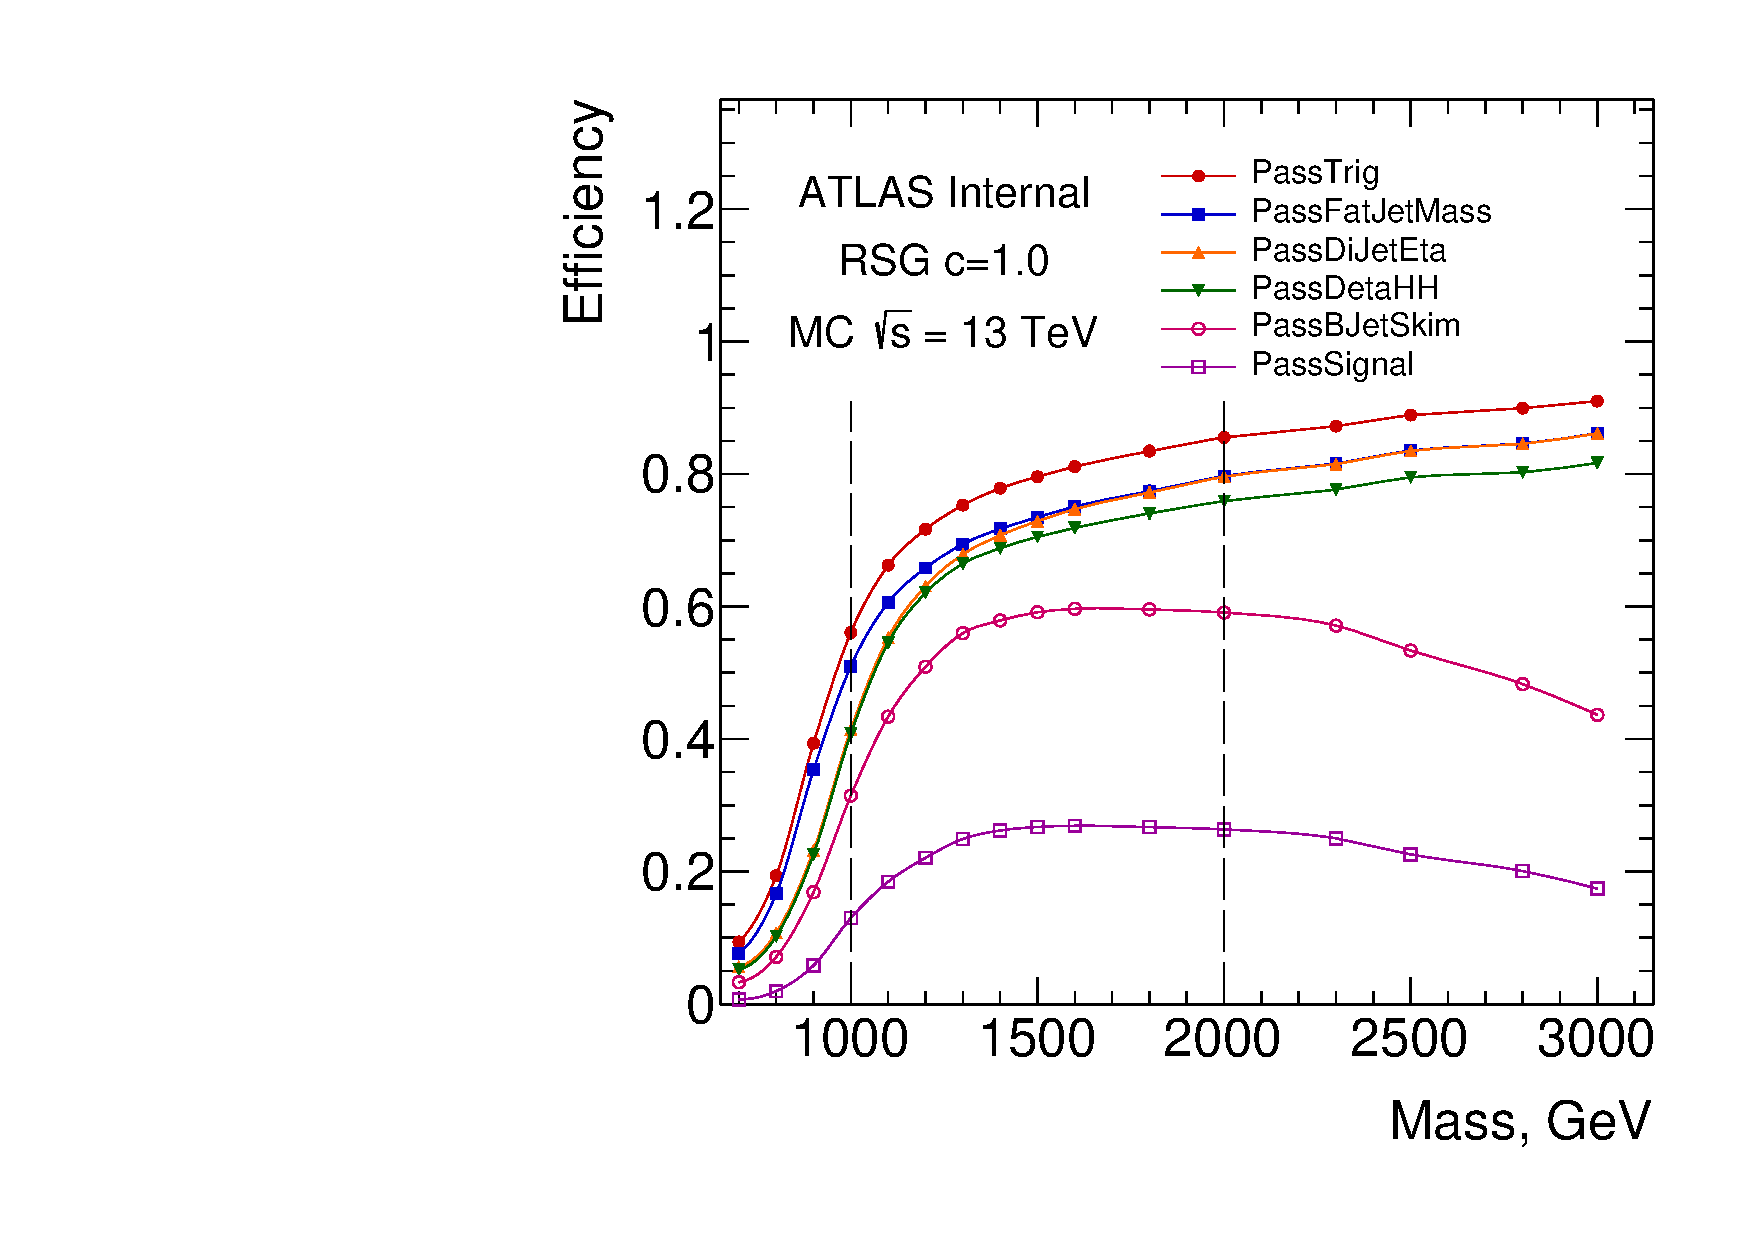
\includegraphics[width=0.48\textwidth,angle=-90]{figures/boosted/SigEff/evtsel_Moriond_Efficiency_PreSel.pdf}
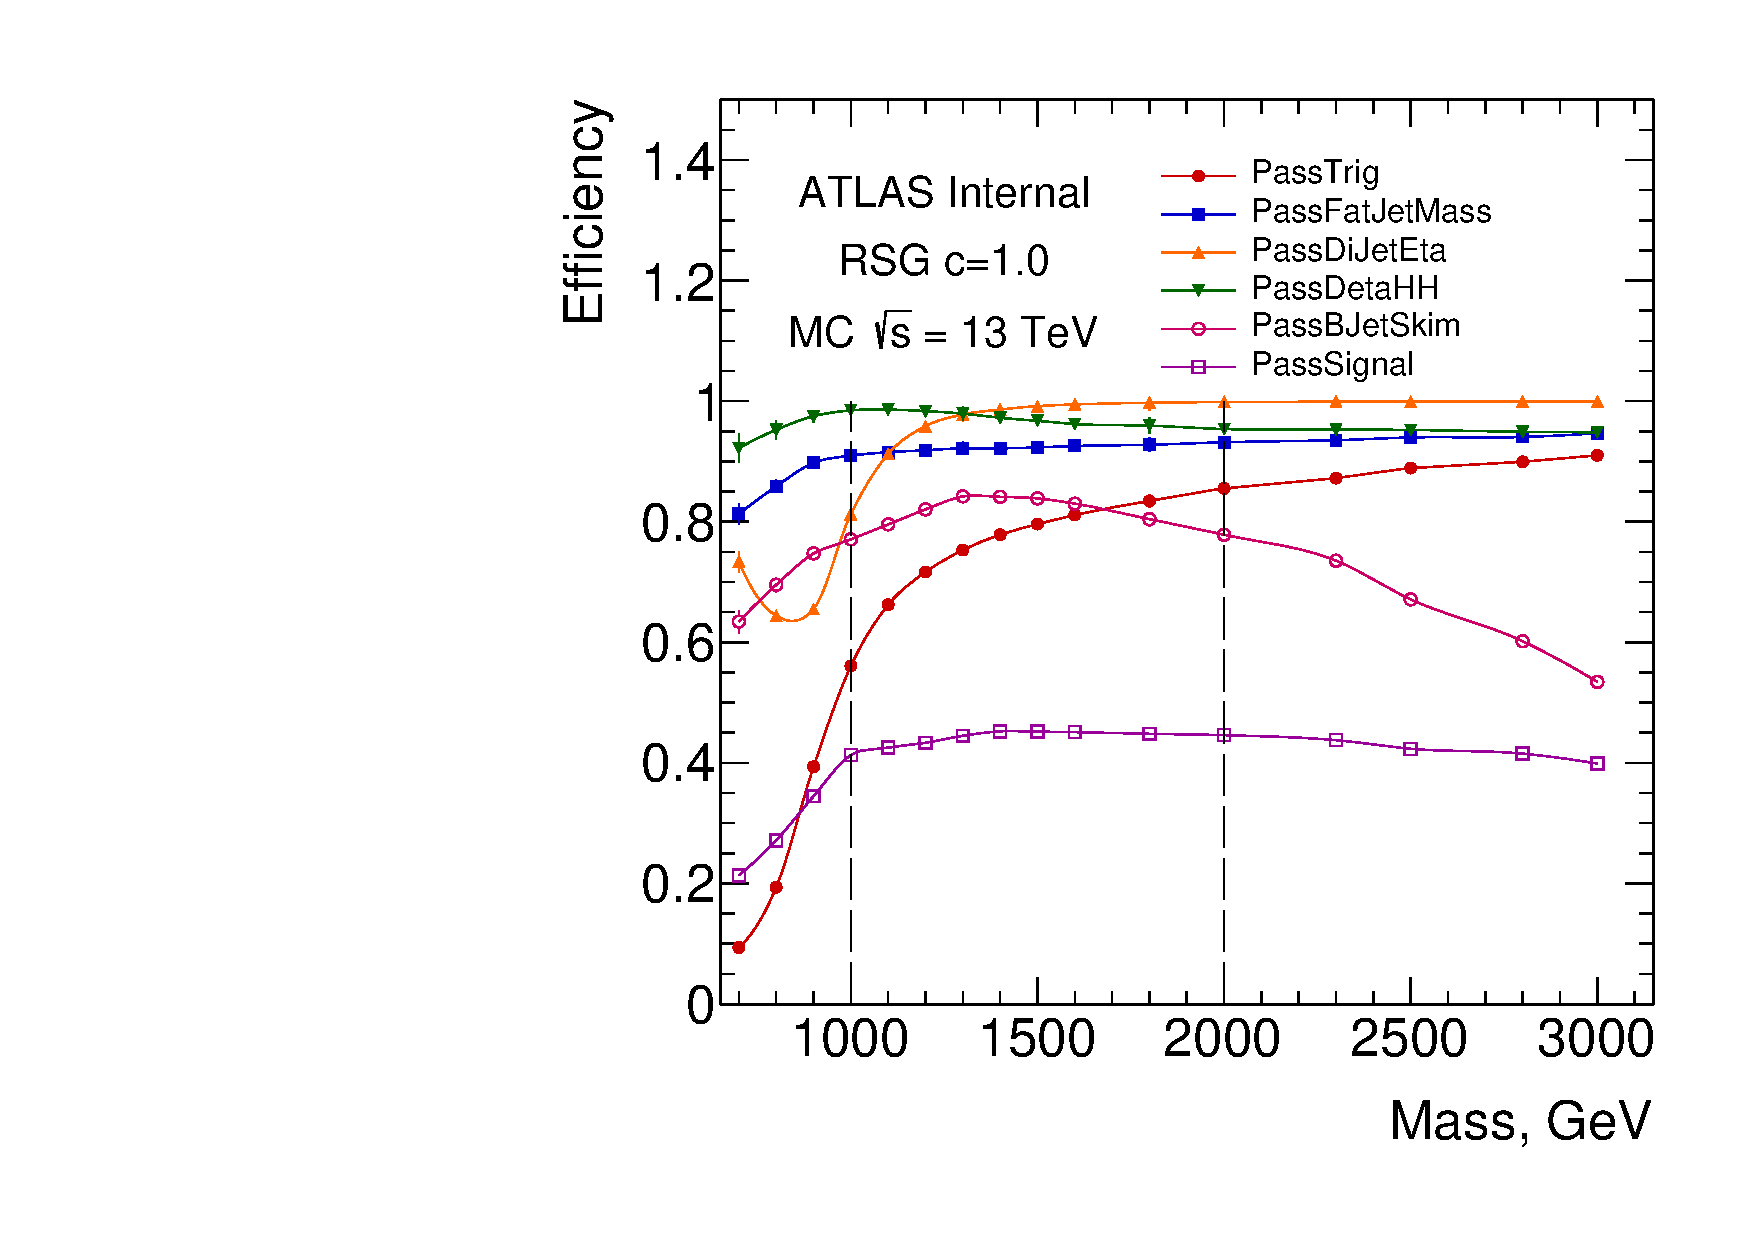
\includegraphics[width=0.48\textwidth,angle=-90]{figures/boosted/SigEff/evtsel_Moriond_Efficiency_PreSel_rel.pdf}
  \caption{Absolute (left) and relative (right) signal efficiency as a function of RSG c=1.0 signal resonance mass hypothesis for selection cuts. The relative efficiency is defined from the previous cut, where the order of cuts is given by the legend. PassTrig means the event passes the trigger selection; PassDiJetPt means the event passes the leading and sub-leading jet \pt cuts; PassDiJetEta means the event passes the leading and sub-leading jet $\eta$ cuts; PassDetaH means the events passes the $|\Delta \eta| < 1.7$ cut; PassBJetSkim means the event contains at least two $b$-tagged track jets, inclusive of 2$b$, 2$b$s, 3$b$ and 4$b$ configurations; PassSignal means the event passes the signal region cut $X_{hh} < 1.6$.}
  \label{fig:boosted-selection-efficiency}
\end{center}
\end{figure*}

\begin{figure*}
\begin{center}
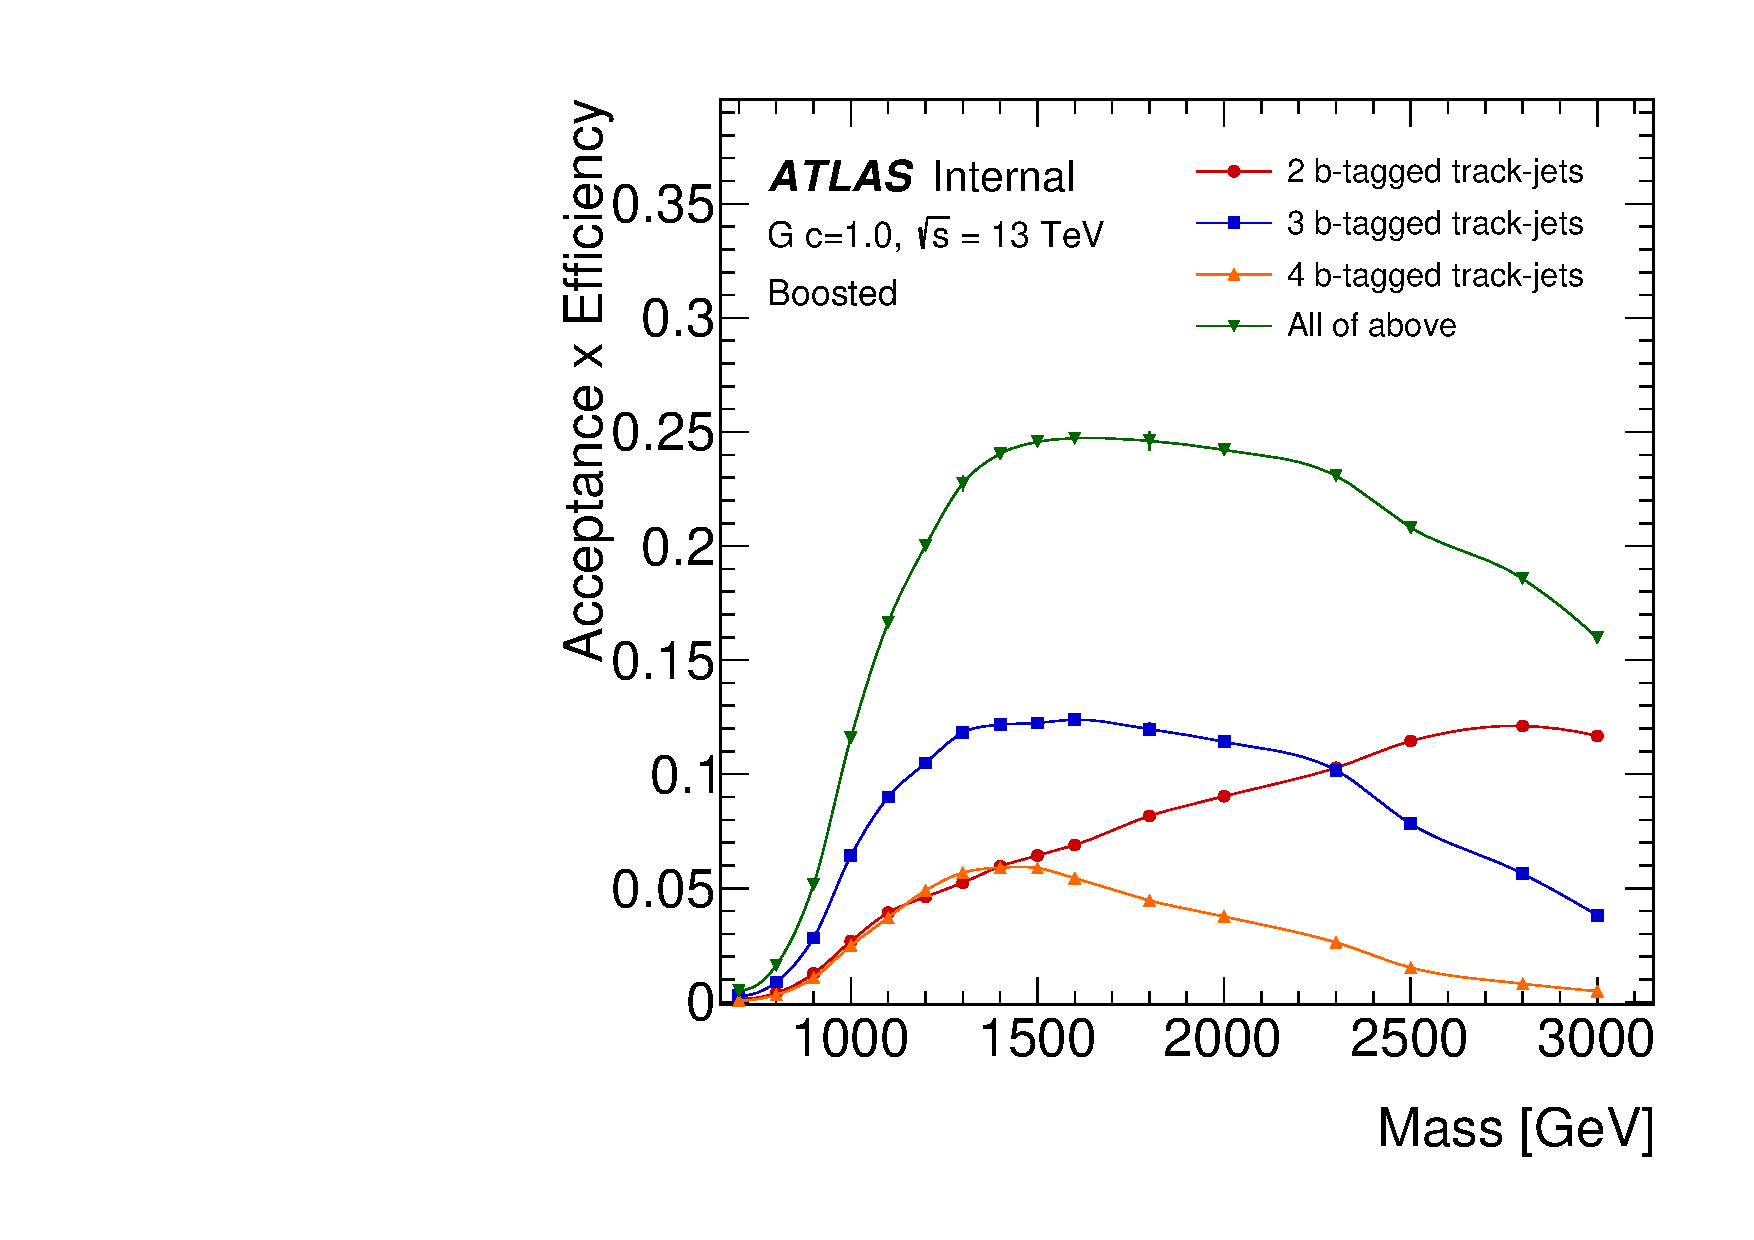
\includegraphics[width=0.48\textwidth,angle=-90]{figures/boosted/SigEff/region_lst_Moriond_bkg_9_Efficiency_PreSel.pdf}
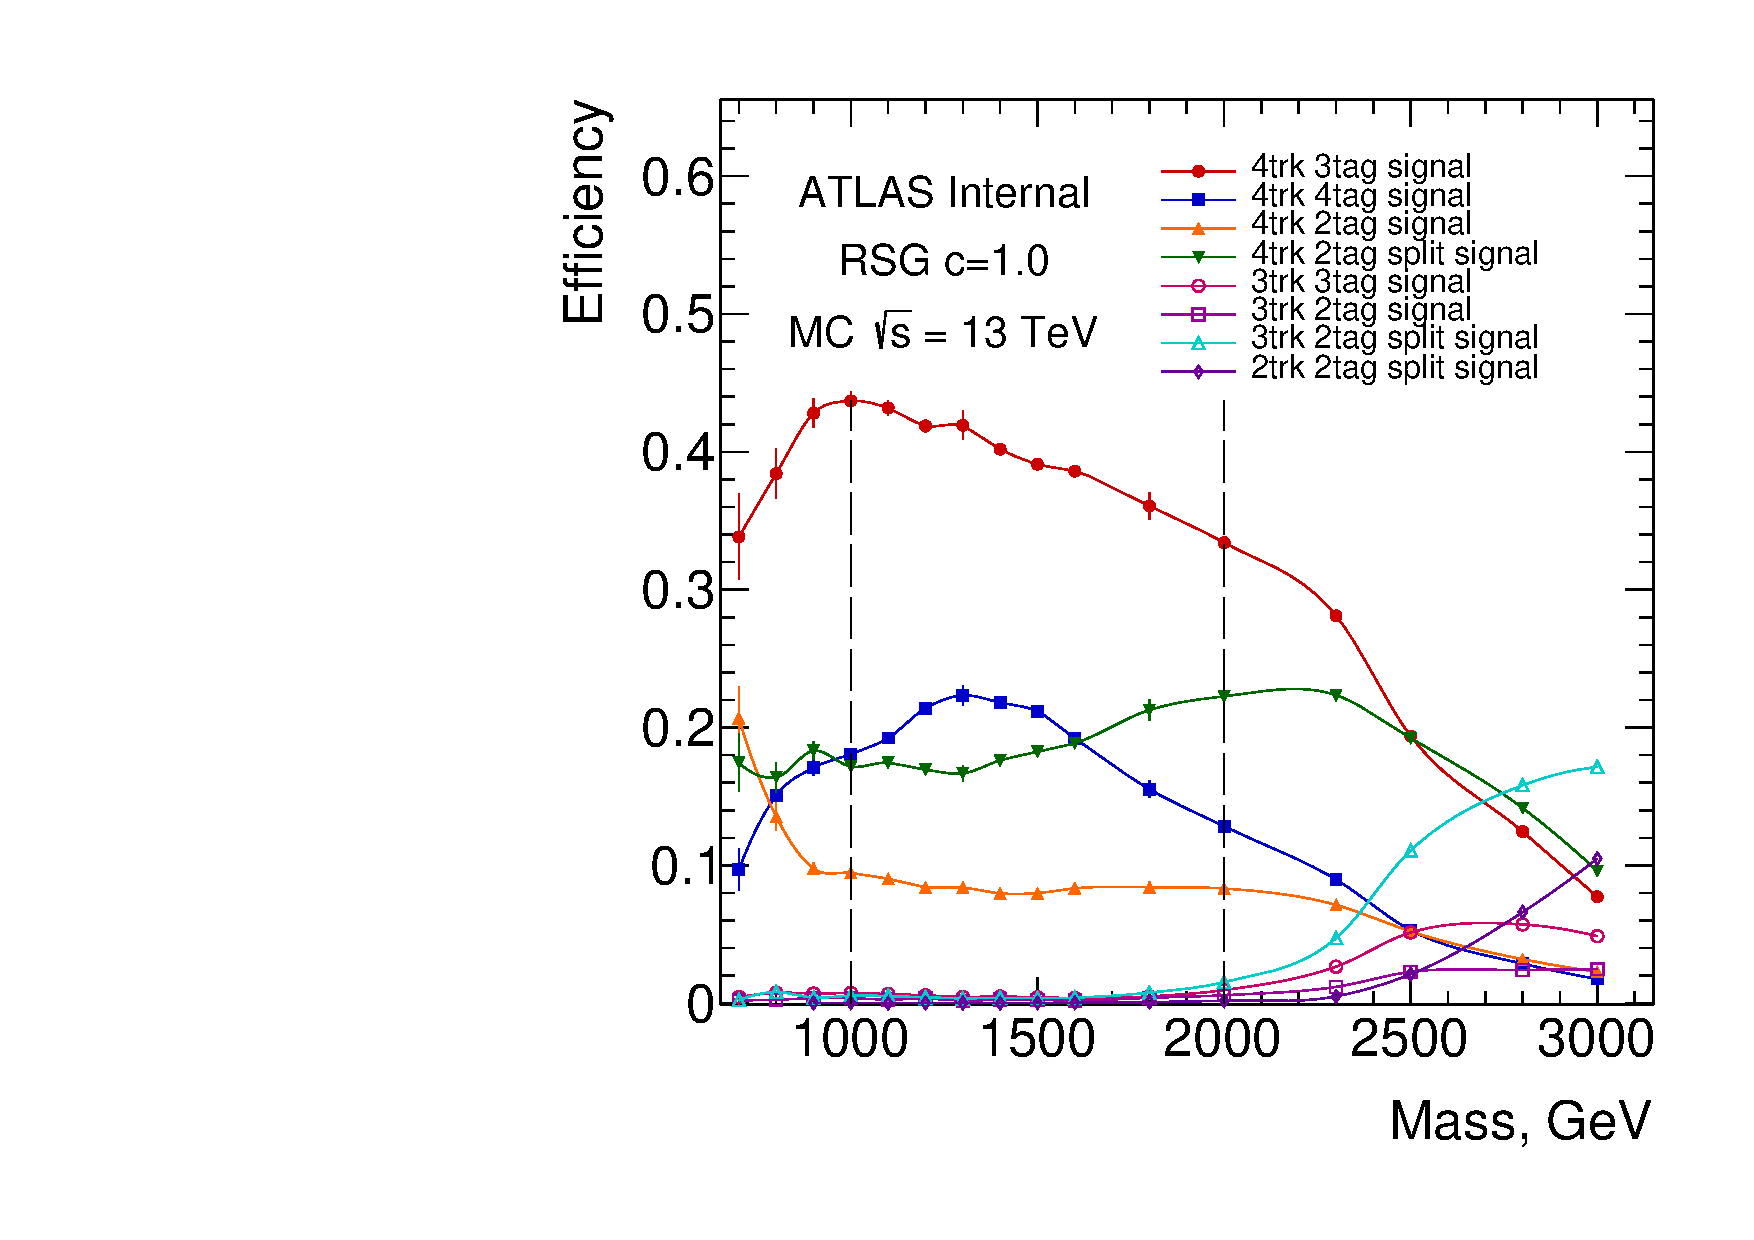
\includegraphics[width=0.48\textwidth,angle=-90]{figures/boosted/SigEff/detail_lst_Moriond_Efficiency_AllTag_Signal.pdf}
%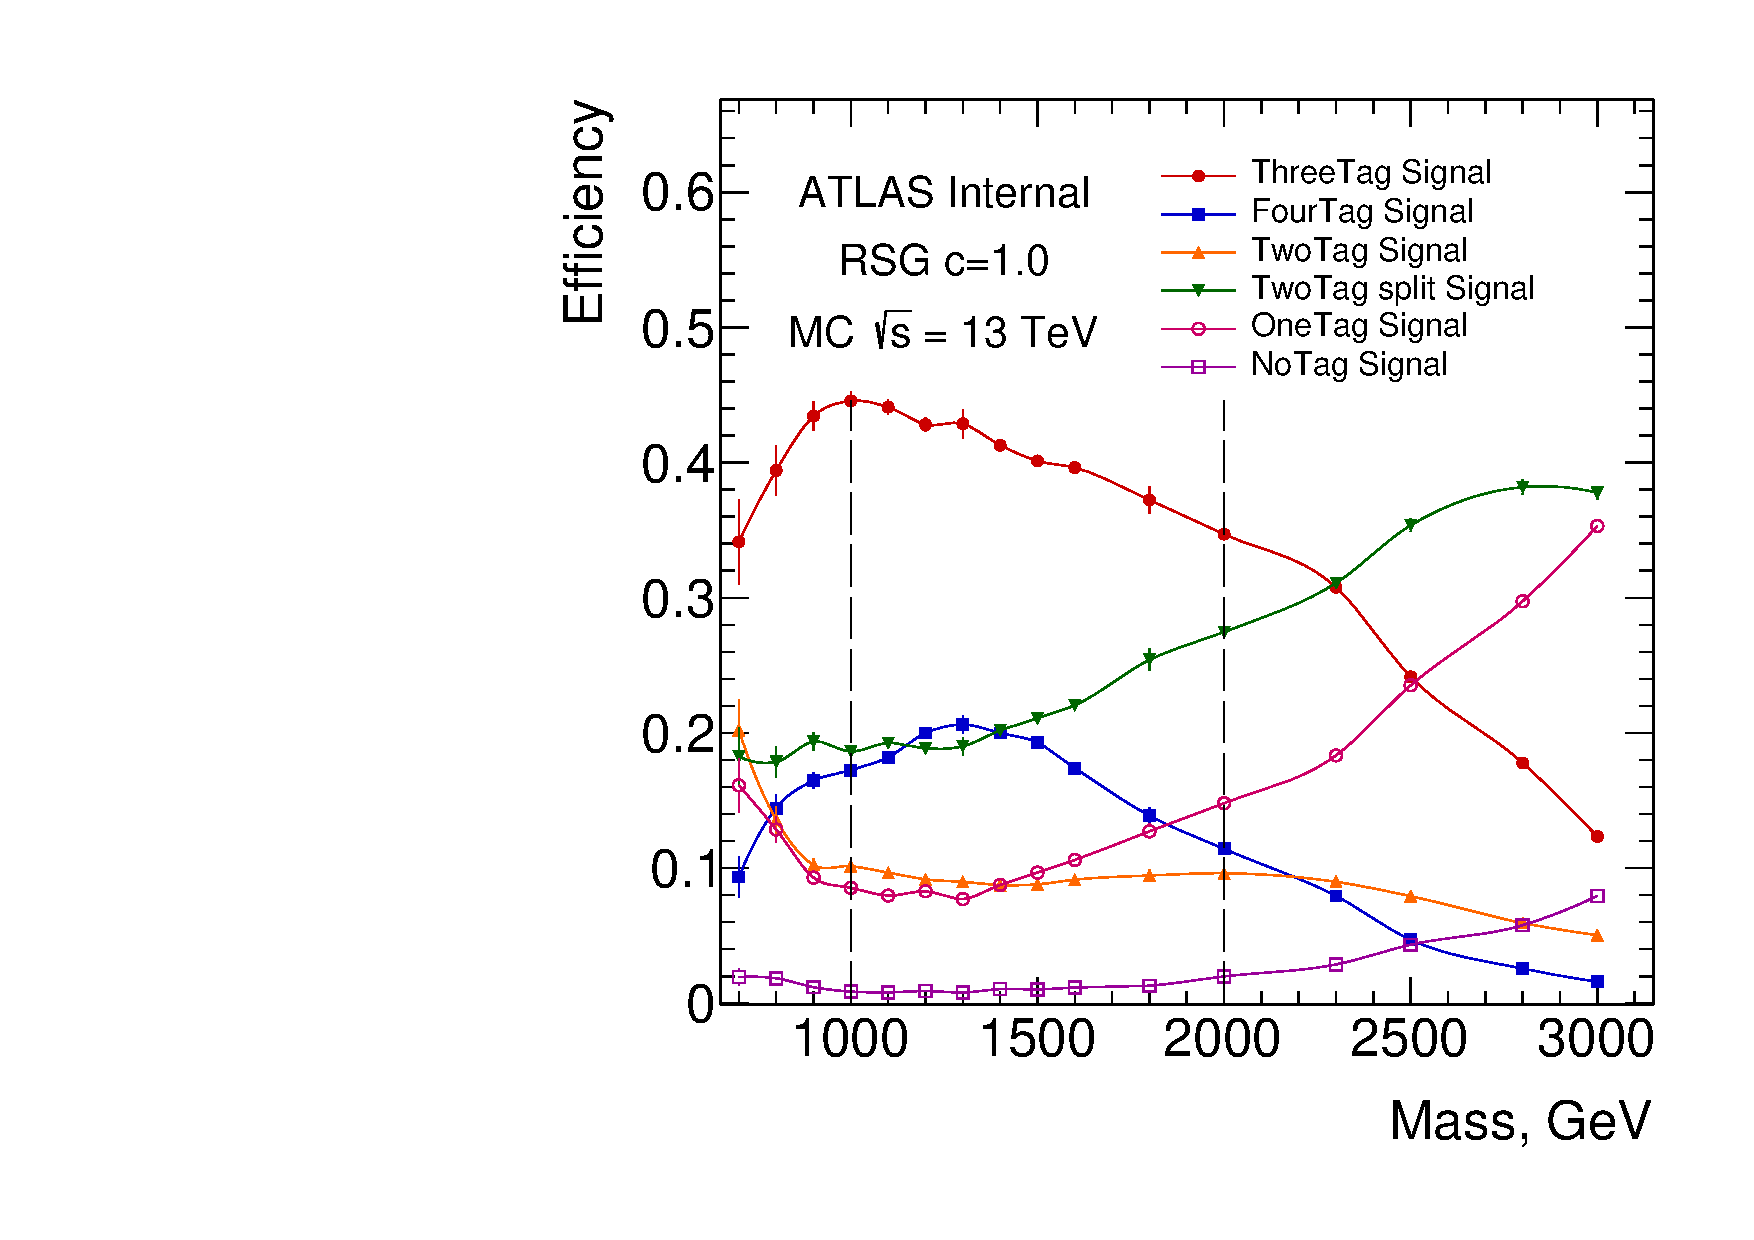
\includegraphics[width=0.48\textwidth,angle=-90]{figures/boosted/SigEff/region_lst_Moriond_Efficiency_AllTag_Signal.pdf}
  \caption{Signal efficiency in three search $b$-tag categories (left) and detailed signal efficiency in different track jet and $b$-tag categories (right) as a function of signal resonance mass hypothesis for selection cuts. The right plot efficiencies are relative to the total number of events in the preselection, whereas the left plot efficiencies are relative to the total number of events in the signal mass region. The green curve in the left plot also corresponds to the PassSignal curve on in Figure ~\ref{fig:boosted-selection-efficiency}.}
  \label{fig:boosted-selection-signal-efficiency}
\end{center}
\end{figure*}

\begin{figure*}
\begin{center}
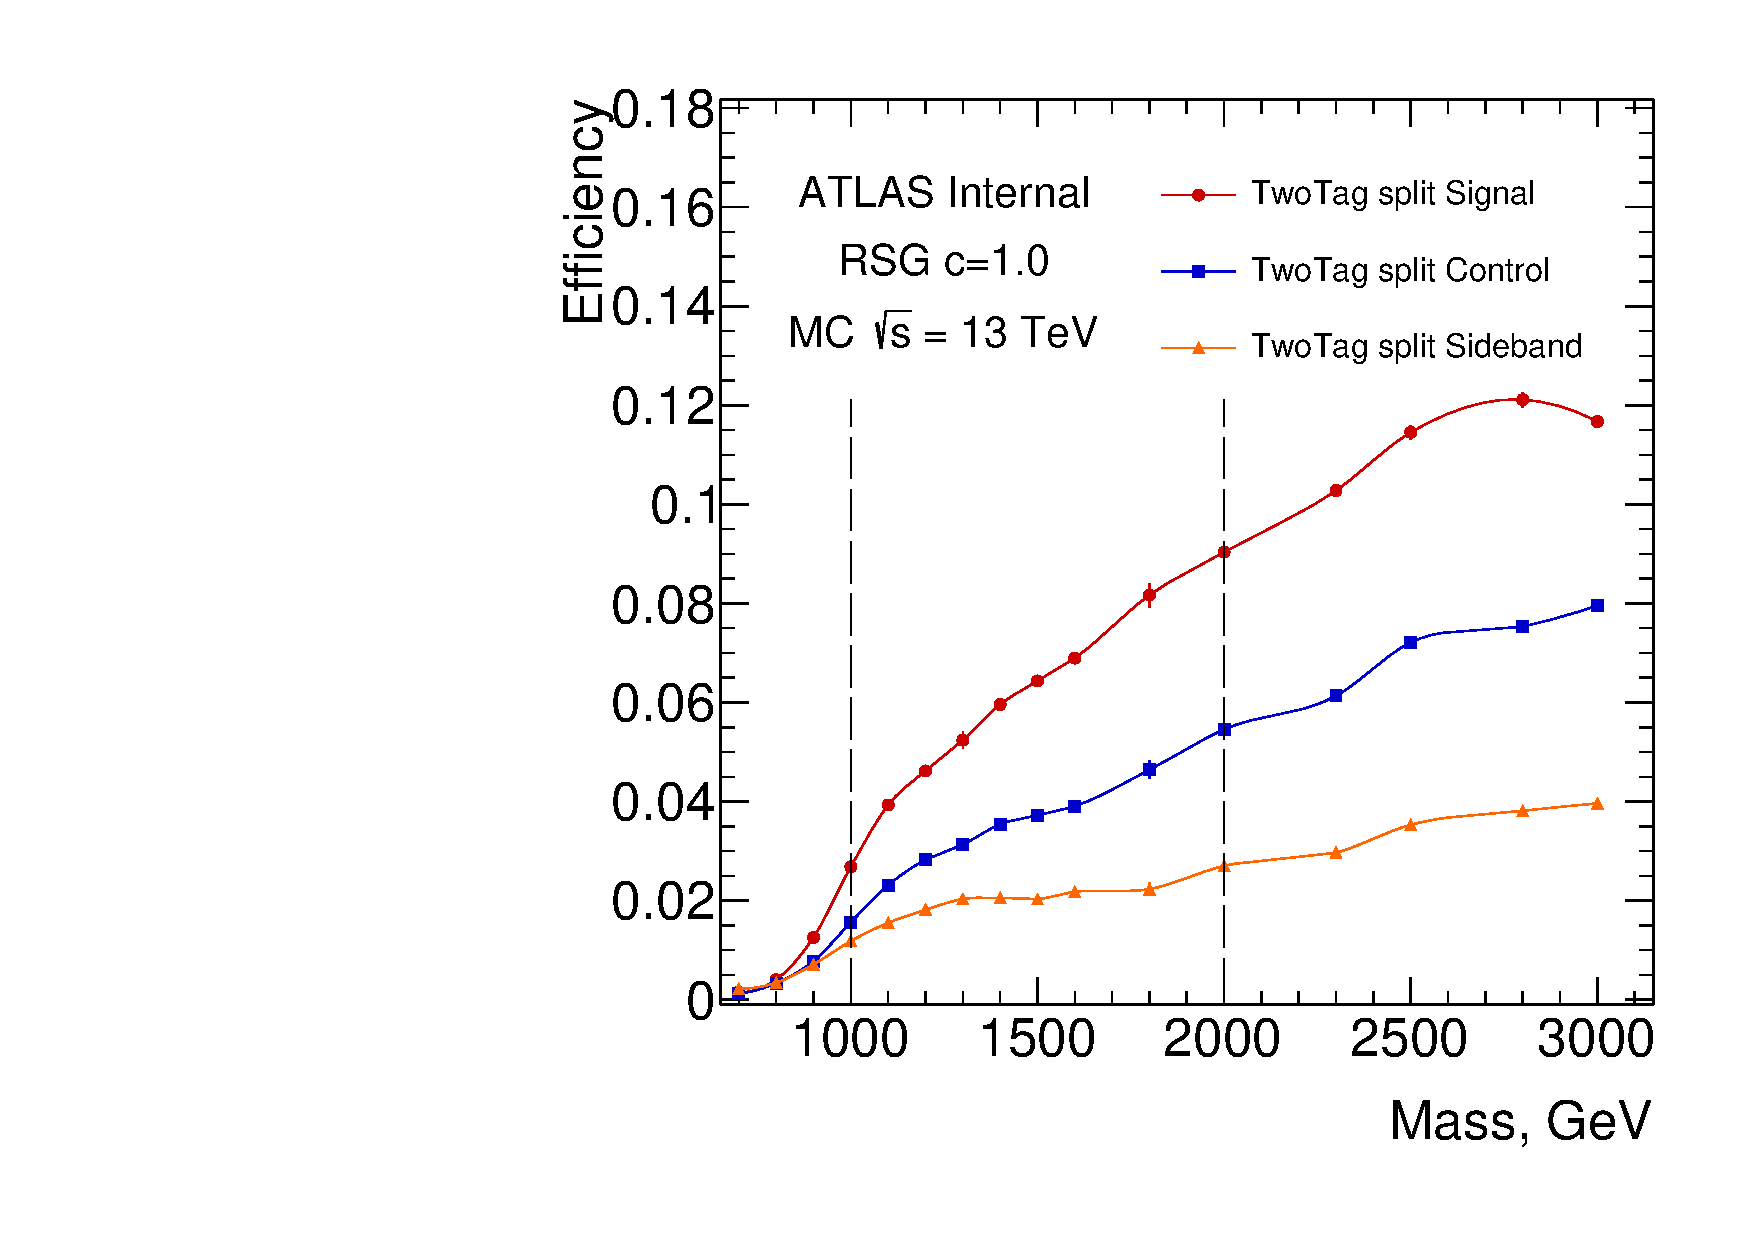
\includegraphics[width=0.48\textwidth,angle=-90]{figures/boosted/SigEff/region_2b_lst_Moriond_Efficiency_PreSel.pdf}
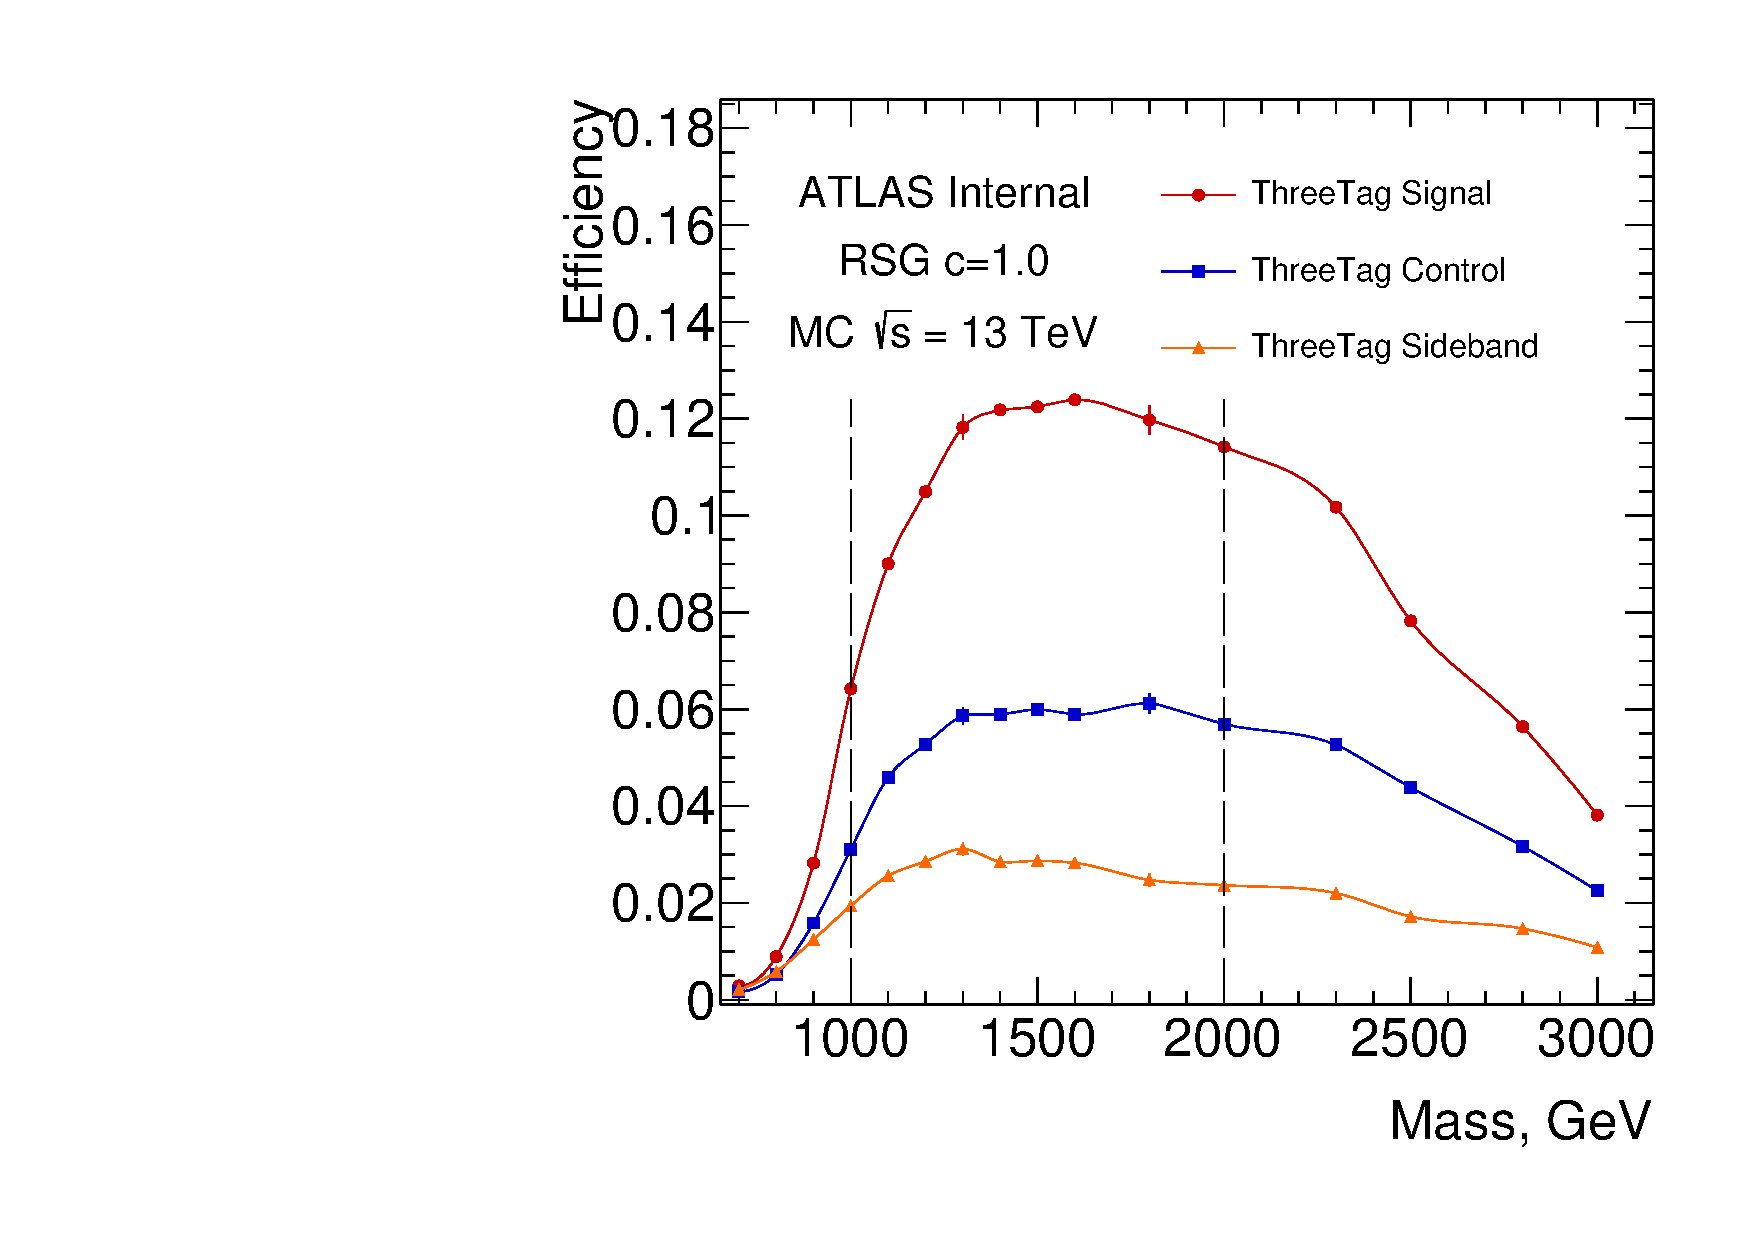
\includegraphics[width=0.48\textwidth,angle=-90]{figures/boosted/SigEff/region_3b_lst_Moriond_Efficiency_PreSel.pdf} \\
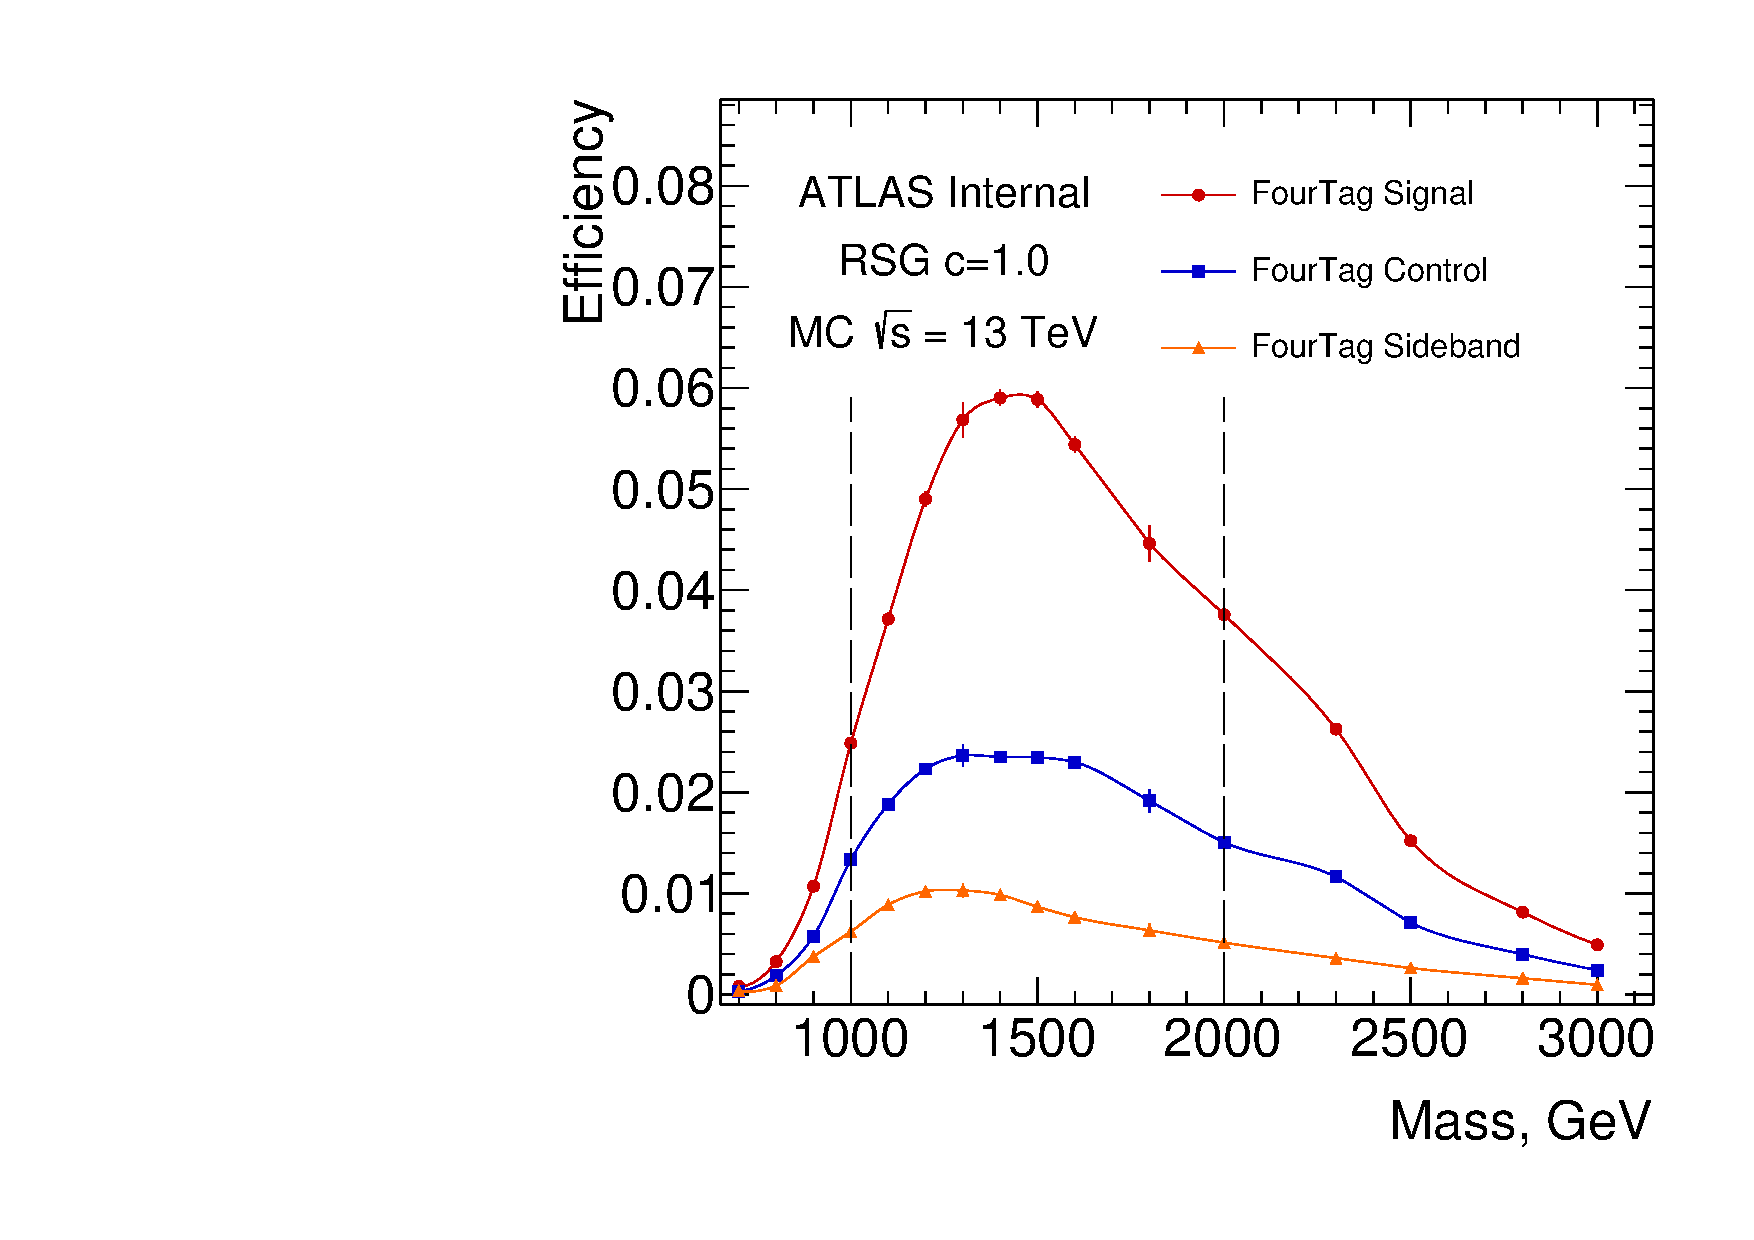
\includegraphics[width=0.48\textwidth,angle=-90]{figures/boosted/SigEff/region_4b_lst_Moriond_Efficiency_PreSel.pdf}
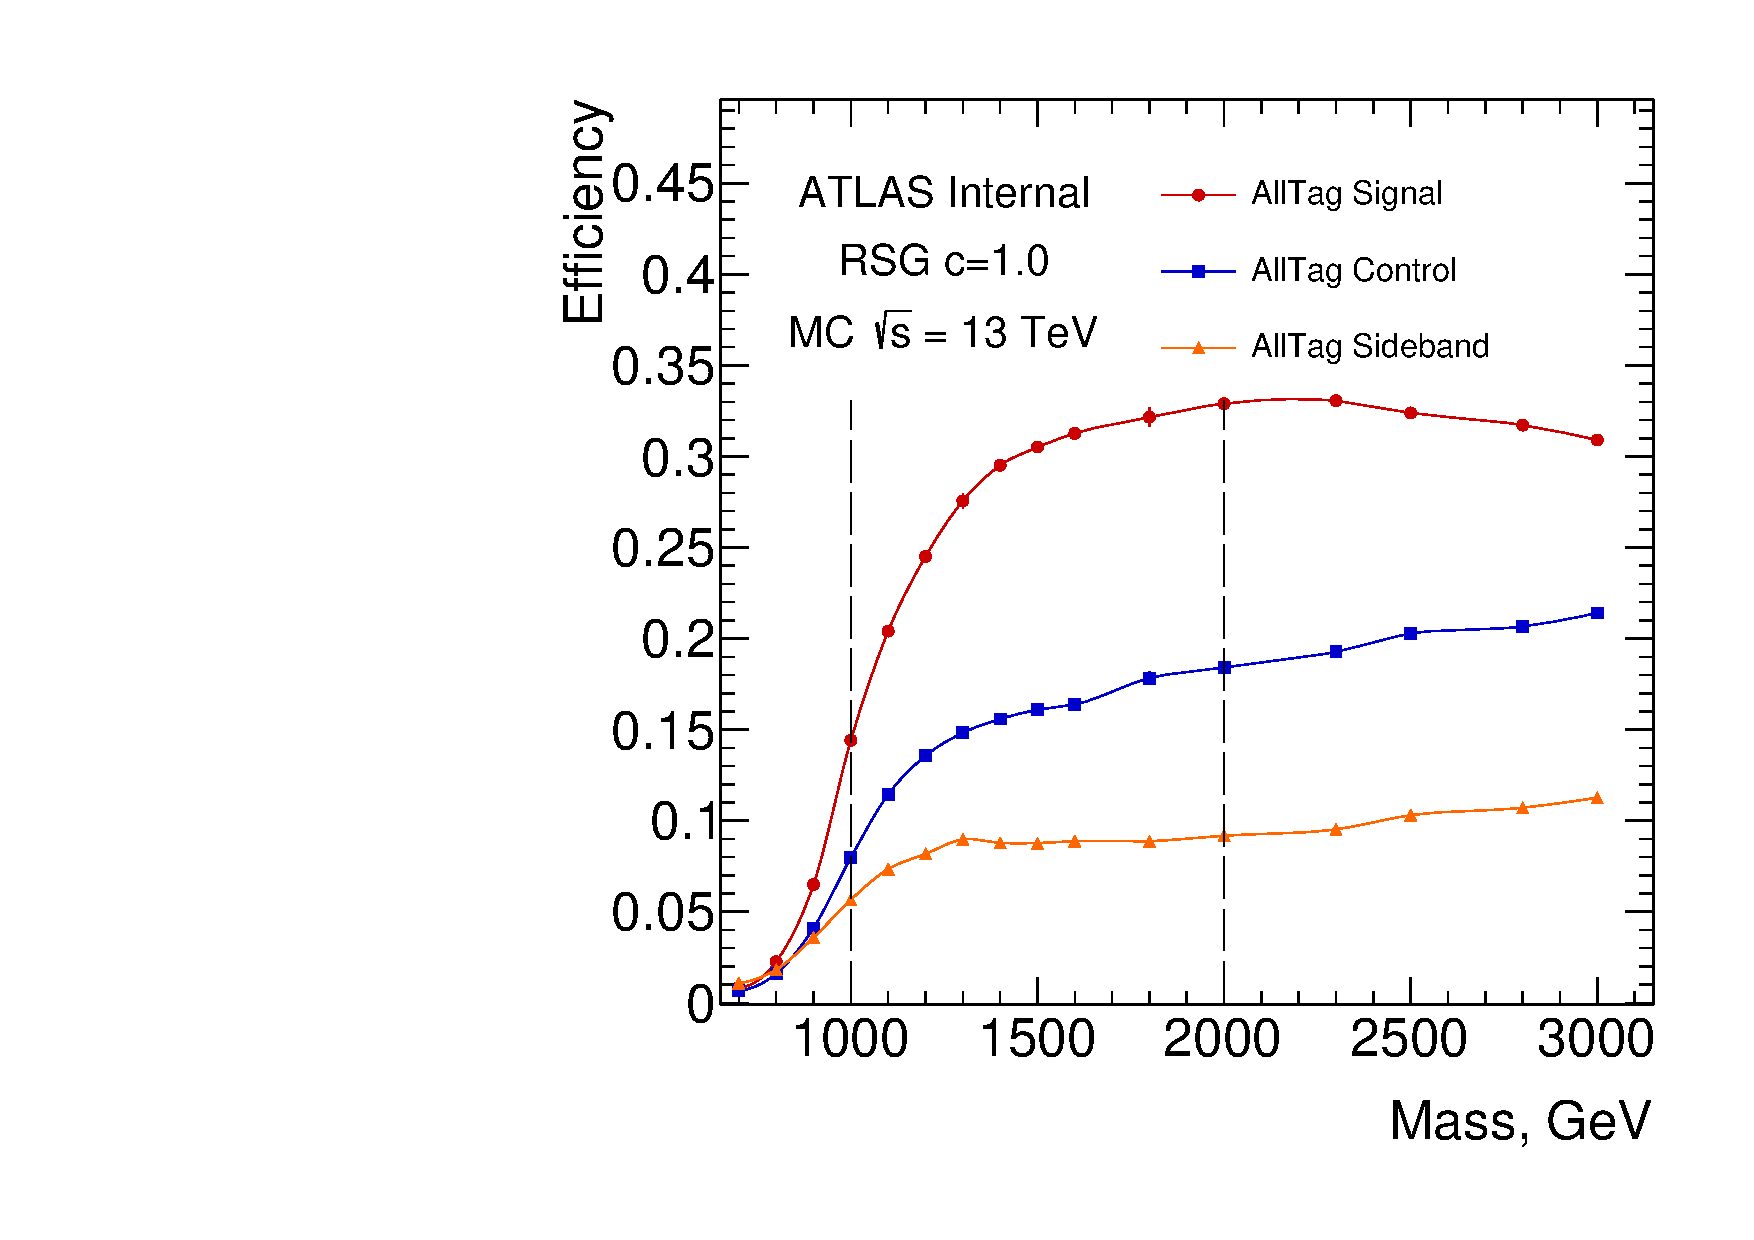
\includegraphics[width=0.48\textwidth,angle=-90]{figures/boosted/SigEff/region_alltag_lst_Moriond_Efficiency_PreSel.pdf} \\
  \caption{Detailed signal efficiency in different signal/control/sideband regions as in 2$b$s (top left, 3$b$ (top right), 4$b$ (bottom left) and inclusive b-tagged regions, which incluse 2$b$, 1$b$ and 0$b$ as well, (bottom right) as a function of signal resonance mass hypothesis for selection cuts. The efficiencies are relative to the total number of events in the preselection.}
  \label{fig:boosted-selection-region-efficiency}
\end{center}
\end{figure*}

%The efficiency of the \texttt{MV2c20} $b$-tagging algorithm is hugely important for the analysis because of the high multiplicity of $b$-jets in the final state. To gauge which working point is best for the analysis, expected sensitivities are derived for various \texttt{MV2c20} working points and described in Appendix~\ref{sec:boosted-optimization}. The 77\% $b$-tag working point is chosen for the analysis.


%%%%%%%%%%%%%%%%%%%%%%%%%%%%%%%%%%%%%%%%%%%%%%%%%%%%%%%%%%%%%%%%%%%%%%%%%%%%%%%%%%%%%%%%%%
\section{Cutflow}
\paragraph{}
Table~\ref{boosted-cutflow} shows the cutflow numbers in data, two different graviton signal MC mass points, $t\bar{t}$ MC samples and $Z+$jets MC samples. The selection efficiency at various stages for RS graviton (RSG) $c=1.0$ (narrow width scalar resonance) signal samples of all mass points can be found in Table~\ref{boosted-eff-RSG_c10}, ~\ref{boosted-eff-RSG_c20} and ~\ref{boosted-eff-2HDM}. Here Sideband indicates the Sideband region as defined before in Equation~\ref{eq:boosted_RhhhighDef}, which is not the whole region outside Control and Signal region.

\begin{table}[htbp!]
\scriptsize
\begin{center}
\resizebox{\textwidth}{!}{
\begin{footnotesize} 
\begin{tabular}{c|c|c|c|c|c|c} 
Cut & Data & $m_{G}=1$TeV & $m_{G}=2$TeV & $m_{G}=3$TeV & $t\bar{t}$ & $Z+jets$ \\ 
\hline\hline 
& & & & & & \\ 
Initial & 23889570.0 $\pm$ 4887.7 & 238.2 $\pm$ 0.98 & 5.72 $\pm$ 0.021 & 0.3 $\pm$ 0.0011 & 210298.2 $\pm$ 415.91 & 35770.71 $\pm$ 365.93\\ 
Pass GRL & 22416007.0 $\pm$ 4734.55 & 238.2 $\pm$ 0.98 & 5.72 $\pm$ 0.021 & 0.3 $\pm$ 0.0011 & 210298.2 $\pm$ 415.91 & 35770.71 $\pm$ 365.93\\ 
Pass Trigger & 21360954.0 $\pm$ 4621.79 & 226.99 $\pm$ 0.96 & 5.71 $\pm$ 0.021 & 0.3 $\pm$ 0.0011 & 190758.37 $\pm$ 392.63 & 30708.09 $\pm$ 329.84\\ 
Pass Jet Cleaning & 21358219.0 $\pm$ 4621.5 & 226.98 $\pm$ 0.96 & 5.71 $\pm$ 0.021 & 0.3 $\pm$ 0.0011 & 190741.16 $\pm$ 392.62 & 30701.46 $\pm$ 329.8\\ 
N(fiducial large-R jets)$\geq 2$ & 21358219.0 $\pm$ 4621.5 & 226.98 $\pm$ 0.96 & 5.71 $\pm$ 0.021 & 0.3 $\pm$ 0.0011 & 190741.16 $\pm$ 392.62 & 30701.46 $\pm$ 329.8\\ 
Pass Large-R jet Selection & 9852994.0 $\pm$ 3138.95 & 167.76 $\pm$ 0.82 & 5.32 $\pm$ 0.02 & 0.29 $\pm$ 0.0011 & 122171.9 $\pm$ 299.65 & 18466.6 $\pm$ 241.77\\ 
$|\Delta\eta(JJ)|<1.7$ & 7671253.0 $\pm$ 2769.7 & 165.2 $\pm$ 0.82 & 5.07 $\pm$ 0.019 & 0.27 $\pm$ 0.0011 & 104353.21 $\pm$ 280.17 & 16879.76 $\pm$ 231.61\\ 
0 b-tags, Sideband & 990693.0 $\pm$ 995.34 & 0.63 $\pm$ 0.054 & 0.029 $\pm$ 0.0016 & 0.0041 $\pm$ 0.00014 & 7562.7 $\pm$ 74.79 & 2634.39 $\pm$ 91.9\\ 
0 b-tags, Control & 401071.0 $\pm$ 633.3 & 0.51 $\pm$ 0.048 & 0.035 $\pm$ 0.0018 & 0.0066 $\pm$ 0.00019 & 1557.48 $\pm$ 33.42 & 1432.14 $\pm$ 67.2\\ 
0 b-tags, Signal & 196205.0 $\pm$ 442.95 & 0.5 $\pm$ 0.048 & 0.044 $\pm$ 0.0021 & 0.0082 $\pm$ 0.00021 & 713.8 $\pm$ 22.77 & 263.61 $\pm$ 29.93\\ 
1 b-tags, Sideband & 269076.0 $\pm$ 518.73 & 3.77 $\pm$ 0.13 & 0.15 $\pm$ 0.0036 & 0.015 $\pm$ 0.00027 & 15677.95 $\pm$ 105.56 & 885.1 $\pm$ 62.2\\ 
1 b-tags, Control & 104862.0 $\pm$ 323.82 & 3.72 $\pm$ 0.13 & 0.23 $\pm$ 0.0045 & 0.026 $\pm$ 0.00036 & 3323.38 $\pm$ 47.64 & 431.92 $\pm$ 44.1\\ 
1 b-tags, Signal & 51791.0 $\pm$ 227.58 & 4.98 $\pm$ 0.15 & 0.33 $\pm$ 0.0055 & 0.036 $\pm$ 0.00042 & 1726.68 $\pm$ 34.02 & 71.72 $\pm$ 18.42\\ 
2 b-tags, Sideband & 28146.0 $\pm$ 167.77 & 3.35 $\pm$ 0.12 & 0.066 $\pm$ 0.0023 & 0.0017 $\pm$ 8.8e-05 & 1249.73 $\pm$ 36.31 & 333.49 $\pm$ 33.25\\ 
2 b-tags, Control & 11204.0 $\pm$ 105.85 & 3.76 $\pm$ 0.13 & 0.12 $\pm$ 0.0032 & 0.0035 $\pm$ 0.00013 & 261.07 $\pm$ 17.22 & 212.37 $\pm$ 32.03\\ 
2 b-tags, Signal & 5495.0 $\pm$ 74.13 & 5.92 $\pm$ 0.16 & 0.21 $\pm$ 0.0042 & 0.0052 $\pm$ 0.00015 & 136.35 $\pm$ 11.5 & 23.94 $\pm$ 10.09\\ 
2 b-tags, split, Sideband & 25137.0 $\pm$ 158.55 & 4.79 $\pm$ 0.14 & 0.18 $\pm$ 0.0039 & 0.013 $\pm$ 0.00025 & 7960.88 $\pm$ 71.27 & 67.74 $\pm$ 16.82\\ 
2 b-tags, split, Control & 8486.0 $\pm$ 92.12 & 6.33 $\pm$ 0.16 & 0.36 $\pm$ 0.0056 & 0.027 $\pm$ 0.00034 & 1505.09 $\pm$ 29.65 & 26.44 $\pm$ 10.08\\ 
2 b-tags, split, Signal &  blinded  & 10.87 $\pm$ 0.22 & 0.6 $\pm$ 0.0072 & 0.039 $\pm$ 0.00041 & 870.13 $\pm$ 22.53 & 0.13 $\pm$ 0.091\\ 
3 b-tags, Sideband & 4403.0 $\pm$ 66.36 & 7.86 $\pm$ 0.18 & 0.16 $\pm$ 0.0035 & 0.0036 $\pm$ 0.00013 & 1066.24 $\pm$ 32.15 & 32.8 $\pm$ 11.34\\ 
3 b-tags, Control & 1553.0 $\pm$ 39.41 & 12.58 $\pm$ 0.23 & 0.38 $\pm$ 0.0054 & 0.0075 $\pm$ 0.00018 & 202.91 $\pm$ 13.94 & 11.21 $\pm$ 5.65\\ 
3 b-tags, Signal &  blinded  & 26.0 $\pm$ 0.33 & 0.76 $\pm$ 0.0076 & 0.013 $\pm$ 0.00023 & 99.18 $\pm$ 10.73 & 0.49 $\pm$ 0.49\\ 
4 b-tags, Sideband & 204.0 $\pm$ 14.28 & 2.52 $\pm$ 0.1 & 0.034 $\pm$ 0.0015 & 0.00032 $\pm$ 3.7e-05 & 31.25 $\pm$ 5.79 & 0 $\pm$ 0\\ 
4 b-tags, Control & 81.0 $\pm$ 9.0 & 5.4 $\pm$ 0.15 & 0.1 $\pm$ 0.0026 & 0.0008 $\pm$ 5.6e-05 & 7.16 $\pm$ 3.31 & 6.18 $\pm$ 5.12\\ 
4 b-tags, Signal &  blinded  & 10.07 $\pm$ 0.2 & 0.25 $\pm$ 0.0041 & 0.0016 $\pm$ 8e-05 & 1.89 $\pm$ 1.37 & 0 $\pm$ 0\\ 
& & & & & & \\ 
\hline\hline 
\end{tabular} 
\end{footnotesize} 
\newline 

}
\end{center}
\caption{Cutflow of data, signal samples of two particular mass points, $t\bar{t}$ and $Z+jets$. Uncertainties are the data/MC stat uncertainty.}
\label{boosted-cutflow}
\end{table}

\begin{table}[htbp!]
\scriptsize
\begin{center}
\resizebox{\textwidth}{!}{
\begin{footnotesize} 
\begin{tabular}{c|c|c|c|c|c|c|c} 
Resonance Mass [GeV] & Mini-ntuple Skimming & 2 large-R jets & $\Delta\eta$ & Xhh < 1.6 & 2bs SR & 3b SR & 4b SR \\ 
\hline\hline 
500 & 317.31 $\pm$ 6.0 & 295.75 $\pm$ 5.79 & 164.5 $\pm$ 4.32 & 8.45 $\pm$ 0.99 & 1.08 $\pm$ 0.37 & 2.14 $\pm$ 0.52 & 0 $\pm$ 0\\ 
600 & 269.07 $\pm$ 3.64 & 247.94 $\pm$ 3.5 & 136.31 $\pm$ 2.59 & 11.31 $\pm$ 0.76 & 2.57 $\pm$ 0.37 & 3.84 $\pm$ 0.45 & 0.66 $\pm$ 0.19\\ 
700 & 253.68 $\pm$ 3.35 & 226.93 $\pm$ 3.16 & 124.83 $\pm$ 2.35 & 16.79 $\pm$ 0.86 & 3.74 $\pm$ 0.42 & 6.99 $\pm$ 0.56 & 1.91 $\pm$ 0.29\\ 
800 & 286.26 $\pm$ 2.28 & 245.36 $\pm$ 2.11 & 129.2 $\pm$ 1.53 & 24.41 $\pm$ 0.67 & 5.11 $\pm$ 0.31 & 11.27 $\pm$ 0.46 & 4.13 $\pm$ 0.27\\ 
900 & 306.51 $\pm$ 1.61 & 275.57 $\pm$ 1.52 & 158.03 $\pm$ 1.15 & 40.72 $\pm$ 0.59 & 8.81 $\pm$ 0.28 & 19.76 $\pm$ 0.41 & 7.5 $\pm$ 0.25\\ 
1000 & 238.2 $\pm$ 0.98 & 226.98 $\pm$ 0.96 & 165.2 $\pm$ 0.82 & 52.86 $\pm$ 0.47 & 10.87 $\pm$ 0.22 & 26.0 $\pm$ 0.33 & 10.07 $\pm$ 0.2\\ 
1100 & 164.5 $\pm$ 0.63 & 160.94 $\pm$ 0.63 & 132.53 $\pm$ 0.57 & 45.26 $\pm$ 0.34 & 9.55 $\pm$ 0.16 & 21.88 $\pm$ 0.23 & 9.03 $\pm$ 0.14\\ 
1200 & 109.24 $\pm$ 0.41 & 107.92 $\pm$ 0.4 & 93.45 $\pm$ 0.38 & 33.53 $\pm$ 0.23 & 6.96 $\pm$ 0.11 & 15.8 $\pm$ 0.16 & 7.38 $\pm$ 0.1\\ 
1300 & 72.72 $\pm$ 0.59 & 72.2 $\pm$ 0.59 & 63.74 $\pm$ 0.56 & 24.19 $\pm$ 0.35 & 5.02 $\pm$ 0.17 & 11.33 $\pm$ 0.24 & 5.45 $\pm$ 0.16\\ 
1400 & 48.83 $\pm$ 0.17 & 48.61 $\pm$ 0.17 & 42.96 $\pm$ 0.16 & 16.62 $\pm$ 0.1 & 3.72 $\pm$ 0.052 & 7.61 $\pm$ 0.07 & 3.68 $\pm$ 0.046\\ 
1500 & 33.13 $\pm$ 0.12 & 33.02 $\pm$ 0.12 & 29.25 $\pm$ 0.11 & 11.31 $\pm$ 0.07 & 2.67 $\pm$ 0.036 & 5.08 $\pm$ 0.047 & 2.44 $\pm$ 0.031\\ 
1600 & 22.81 $\pm$ 0.08 & 22.75 $\pm$ 0.08 & 20.16 $\pm$ 0.075 & 7.74 $\pm$ 0.048 & 1.93 $\pm$ 0.025 & 3.48 $\pm$ 0.032 & 1.53 $\pm$ 0.02\\ 
1800 & 11.2 $\pm$ 0.1 & 11.18 $\pm$ 0.1 & 9.93 $\pm$ 0.094 & 3.71 $\pm$ 0.059 & 1.1 $\pm$ 0.034 & 1.6 $\pm$ 0.038 & 0.6 $\pm$ 0.022\\ 
2000 & 5.72 $\pm$ 0.021 & 5.71 $\pm$ 0.021 & 5.07 $\pm$ 0.019 & 1.83 $\pm$ 0.012 & 0.6 $\pm$ 0.0072 & 0.76 $\pm$ 0.0076 & 0.25 $\pm$ 0.0041\\ 
2250 & 2.61 $\pm$ 0.0088 & 2.61 $\pm$ 0.0088 & 2.32 $\pm$ 0.0083 & 0.78 $\pm$ 0.005 & 0.31 $\pm$ 0.0032 & 0.3 $\pm$ 0.003 & 0.078 $\pm$ 0.0014\\ 
2500 & 1.24 $\pm$ 0.0054 & 1.24 $\pm$ 0.0054 & 1.11 $\pm$ 0.0051 & 0.33 $\pm$ 0.0028 & 0.16 $\pm$ 0.002 & 0.11 $\pm$ 0.0016 & 0.021 $\pm$ 0.00066\\ 
2750 & 0.6 $\pm$ 0.0026 & 0.6 $\pm$ 0.0026 & 0.54 $\pm$ 0.0025 & 0.14 $\pm$ 0.0013 & 0.081 $\pm$ 0.00099 & 0.038 $\pm$ 0.00065 & 0.0055 $\pm$ 0.00024\\ 
3000 & 0.3 $\pm$ 0.0011 & 0.3 $\pm$ 0.0011 & 0.27 $\pm$ 0.0011 & 0.058 $\pm$ 0.00051 & 0.039 $\pm$ 0.00041 & 0.013 $\pm$ 0.00023 & 0.0016 $\pm$ 8e-05\\ 
\hline\hline 
\end{tabular} 
\end{footnotesize} 
\newline 

}
\end{center}
\caption{The selection efficiency for $G_{KK}^{*}\rightarrow hh\rightarrow b\bar{b}b\bar{b}$ events ($c=1.0$) at each stage of the event selection. Uncertainties are the MC stat uncertainty only.}
\label{boosted-eff-RSG_c10}
\end{table}

\begin{table}[htbp!]
\scriptsize
\begin{center}
\resizebox{\textwidth}{!}{
\begin{footnotesize} 
\begin{tabular}{c|c|c|c|c|c|c|c} 
Resonance Mass [GeV] & Mini-ntuple Skimming & 2 large-R jets & $\Delta\eta$ & Xhh < 1.6 & 2bs SR & 3b SR & 4b SR \\ 
\hline\hline 
500 & 3705.15 $\pm$ 40.86 & 3479.44 $\pm$ 39.59 & 2325.18 $\pm$ 32.37 & 568.04 $\pm$ 16.17 & 122.56 $\pm$ 7.76 & 253.49 $\pm$ 10.78 & 100.7 $\pm$ 6.53\\ 
600 & 2549.14 $\pm$ 22.55 & 2374.01 $\pm$ 21.76 & 1591.92 $\pm$ 17.82 & 396.96 $\pm$ 9.03 & 89.01 $\pm$ 4.46 & 178.63 $\pm$ 6.05 & 74.31 $\pm$ 3.71\\ 
700 & 1928.4 $\pm$ 13.57 & 1782.85 $\pm$ 13.04 & 1183.86 $\pm$ 10.63 & 320.53 $\pm$ 5.62 & 71.38 $\pm$ 2.76 & 148.41 $\pm$ 3.81 & 59.31 $\pm$ 2.31\\ 
800 & 1595.14 $\pm$ 8.82 & 1457.71 $\pm$ 8.43 & 958.89 $\pm$ 6.84 & 268.75 $\pm$ 3.67 & 64.14 $\pm$ 1.86 & 123.48 $\pm$ 2.47 & 49.43 $\pm$ 1.51\\ 
900 & 1264.78 $\pm$ 5.77 & 1179.88 $\pm$ 5.58 & 819.75 $\pm$ 4.65 & 251.29 $\pm$ 2.61 & 55.63 $\pm$ 1.27 & 119.44 $\pm$ 1.79 & 48.72 $\pm$ 1.11\\ 
1000 & 891.0 $\pm$ 3.66 & 856.95 $\pm$ 3.59 & 662.54 $\pm$ 3.15 & 219.04 $\pm$ 1.84 & 49.45 $\pm$ 0.91 & 104.31 $\pm$ 1.26 & 42.97 $\pm$ 0.78\\ 
1100 & 595.58 $\pm$ 2.98 & 581.72 $\pm$ 2.95 & 481.67 $\pm$ 2.68 & 167.96 $\pm$ 1.61 & 37.64 $\pm$ 0.79 & 78.28 $\pm$ 1.09 & 34.59 $\pm$ 0.7\\ 
1200 & 390.84 $\pm$ 1.69 & 385.41 $\pm$ 1.68 & 330.23 $\pm$ 1.55 & 118.0 $\pm$ 0.94 & 26.23 $\pm$ 0.46 & 54.18 $\pm$ 0.64 & 25.34 $\pm$ 0.42\\ 
1300 & 257.66 $\pm$ 0.94 & 255.35 $\pm$ 0.94 & 222.37 $\pm$ 0.88 & 82.11 $\pm$ 0.54 & 19.04 $\pm$ 0.27 & 37.8 $\pm$ 0.37 & 16.99 $\pm$ 0.23\\ 
1400 & 172.09 $\pm$ 0.72 & 171.02 $\pm$ 0.71 & 150.22 $\pm$ 0.67 & 56.23 $\pm$ 0.42 & 13.6 $\pm$ 0.22 & 25.36 $\pm$ 0.28 & 11.78 $\pm$ 0.18\\ 
1500 & 116.25 $\pm$ 0.41 & 115.72 $\pm$ 0.41 & 101.92 $\pm$ 0.39 & 38.5 $\pm$ 0.24 & 9.94 $\pm$ 0.13 & 17.04 $\pm$ 0.16 & 7.64 $\pm$ 0.1\\ 
1600 & 80.09 $\pm$ 0.28 & 79.82 $\pm$ 0.28 & 70.48 $\pm$ 0.26 & 26.24 $\pm$ 0.16 & 7.01 $\pm$ 0.09 & 11.62 $\pm$ 0.11 & 4.92 $\pm$ 0.067\\ 
1800 & 38.99 $\pm$ 0.14 & 38.9 $\pm$ 0.14 & 34.39 $\pm$ 0.13 & 12.65 $\pm$ 0.081 & 3.82 $\pm$ 0.047 & 5.46 $\pm$ 0.053 & 2.02 $\pm$ 0.03\\ 
2000 & 19.94 $\pm$ 0.088 & 19.91 $\pm$ 0.088 & 17.68 $\pm$ 0.083 & 6.17 $\pm$ 0.05 & 2.15 $\pm$ 0.031 & 2.52 $\pm$ 0.032 & 0.85 $\pm$ 0.017\\ 
2250 & 9.02 $\pm$ 0.031 & 9.01 $\pm$ 0.031 & 7.99 $\pm$ 0.029 & 2.62 $\pm$ 0.017 & 1.03 $\pm$ 0.011 & 1.02 $\pm$ 0.01 & 0.28 $\pm$ 0.0051\\ 
2500 & 4.28 $\pm$ 0.016 & 4.28 $\pm$ 0.016 & 3.8 $\pm$ 0.015 & 1.13 $\pm$ 0.0083 & 0.52 $\pm$ 0.0058 & 0.4 $\pm$ 0.0048 & 0.098 $\pm$ 0.0022\\ 
3000 & 1.07 $\pm$ 0.004 & 1.07 $\pm$ 0.004 & 0.96 $\pm$ 0.0038 & 0.23 $\pm$ 0.0019 & 0.13 $\pm$ 0.0015 & 0.062 $\pm$ 0.00097 & 0.013 $\pm$ 0.00043\\ 
\hline\hline 
\end{tabular} 
\end{footnotesize} 
\newline 

}
\end{center}
\caption{The selection efficiency for $G_{KK}^{*}\rightarrow hh\rightarrow b\bar{b}b\bar{b}$ events ($c=2.0$) at each stage of the event selection. Uncertainties are the MC stat uncertainty only.}
\label{boosted-eff-RSG_c20}
\end{table}

\begin{table}[htbp!]
\scriptsize
\begin{center}
\resizebox{\textwidth}{!}{
\begin{footnotesize} 
\begin{tabular}{c|c|c|c|c|c|c|c} 
Resonance Mass [GeV] & Mini-ntuple Skimming & 2 large-R jets & $\Delta\eta$ & Xhh < 1.6 & 2bs SR & 3b SR & 4b SR \\ 
\hline\hline 
500 & 1557.94 $\pm$ 136.12 & 1022.77 $\pm$ 110.29 & 95.14 $\pm$ 33.64 & 11.69 $\pm$ 11.69 & 0 $\pm$ 0 & 11.69 $\pm$ 11.69 & 0 $\pm$ 0\\ 
600 & 3289.78 $\pm$ 123.99 & 2542.11 $\pm$ 108.99 & 485.99 $\pm$ 47.66 & 54.55 $\pm$ 15.77 & 18.73 $\pm$ 9.39 & 9.17 $\pm$ 6.49 & 0 $\pm$ 0\\ 
700 & 4655.21 $\pm$ 94.59 & 3855.64 $\pm$ 86.09 & 1237.8 $\pm$ 48.78 & 142.42 $\pm$ 17.03 & 28.55 $\pm$ 7.74 & 52.6 $\pm$ 10.75 & 7.69 $\pm$ 3.85\\ 
800 & 7506.31 $\pm$ 81.79 & 6020.56 $\pm$ 73.25 & 2150.64 $\pm$ 43.78 & 320.63 $\pm$ 17.02 & 67.63 $\pm$ 7.83 & 139.97 $\pm$ 11.23 & 47.57 $\pm$ 6.75\\ 
900 & 9732.89 $\pm$ 61.17 & 8400.91 $\pm$ 56.83 & 3574.63 $\pm$ 37.07 & 806.13 $\pm$ 17.76 & 188.71 $\pm$ 8.71 & 377.92 $\pm$ 12.12 & 127.7 $\pm$ 6.99\\ 
1000 & 7516.07 $\pm$ 37.72 & 7033.18 $\pm$ 36.49 & 4496.85 $\pm$ 29.18 & 1351.1 $\pm$ 16.2 & 303.71 $\pm$ 7.88 & 650.89 $\pm$ 11.19 & 234.2 $\pm$ 6.57\\ 
1100 & 4731.39 $\pm$ 21.54 & 4563.4 $\pm$ 21.15 & 3485.58 $\pm$ 18.49 & 1135.18 $\pm$ 10.7 & 251.77 $\pm$ 5.18 & 539.51 $\pm$ 7.36 & 215.39 $\pm$ 4.5\\ 
1200 & 2853.51 $\pm$ 12.23 & 2782.42 $\pm$ 12.07 & 2253.95 $\pm$ 10.87 & 786.92 $\pm$ 6.53 & 175.53 $\pm$ 3.21 & 366.01 $\pm$ 4.44 & 158.29 $\pm$ 2.8\\ 
1300 & 1700.83 $\pm$ 7.01 & 1668.05 $\pm$ 6.94 & 1362.91 $\pm$ 6.27 & 494.36 $\pm$ 3.84 & 107.0 $\pm$ 1.86 & 224.19 $\pm$ 2.58 & 107.55 $\pm$ 1.7\\ 
1400 & 1016.14 $\pm$ 4.03 & 999.98 $\pm$ 4.0 & 802.44 $\pm$ 3.59 & 296.46 $\pm$ 2.22 & 65.49 $\pm$ 1.1 & 133.86 $\pm$ 1.49 & 65.58 $\pm$ 0.99\\ 
1500 & 621.34 $\pm$ 2.41 & 613.46 $\pm$ 2.39 & 484.92 $\pm$ 2.13 & 179.29 $\pm$ 1.32 & 42.75 $\pm$ 0.68 & 79.32 $\pm$ 0.88 & 36.77 $\pm$ 0.56\\ 
1600 & 386.3 $\pm$ 1.46 & 382.44 $\pm$ 1.46 & 297.63 $\pm$ 1.28 & 109.99 $\pm$ 0.8 & 27.68 $\pm$ 0.42 & 49.3 $\pm$ 0.53 & 20.92 $\pm$ 0.32\\ 
1800 & 154.8 $\pm$ 0.58 & 153.5 $\pm$ 0.57 & 116.52 $\pm$ 0.5 & 42.24 $\pm$ 0.31 & 12.41 $\pm$ 0.18 & 18.2 $\pm$ 0.2 & 6.66 $\pm$ 0.11\\ 
2000 & 65.4 $\pm$ 0.24 & 65.02 $\pm$ 0.24 & 48.57 $\pm$ 0.2 & 16.89 $\pm$ 0.12 & 5.64 $\pm$ 0.076 & 7.01 $\pm$ 0.079 & 2.18 $\pm$ 0.041\\ 
2250 & 23.84 $\pm$ 0.085 & 23.73 $\pm$ 0.085 & 17.44 $\pm$ 0.073 & 5.57 $\pm$ 0.042 & 2.25 $\pm$ 0.028 & 2.11 $\pm$ 0.025 & 0.52 $\pm$ 0.012\\ 
2500 & 9.2 $\pm$ 0.032 & 9.17 $\pm$ 0.032 & 6.72 $\pm$ 0.028 & 1.9 $\pm$ 0.015 & 0.92 $\pm$ 0.011 & 0.64 $\pm$ 0.0086 & 0.11 $\pm$ 0.0034\\ 
2750 & 3.73 $\pm$ 0.013 & 3.73 $\pm$ 0.013 & 2.71 $\pm$ 0.011 & 0.63 $\pm$ 0.0054 & 0.37 $\pm$ 0.0042 & 0.17 $\pm$ 0.0027 & 0.021 $\pm$ 0.00093\\ 
3000 & 1.59 $\pm$ 0.0054 & 1.59 $\pm$ 0.0054 & 1.15 $\pm$ 0.0046 & 0.22 $\pm$ 0.0021 & 0.15 $\pm$ 0.0017 & 0.044 $\pm$ 0.0009 & 0.0038 $\pm$ 0.00025\\ 
\hline\hline 
\end{tabular} 
\end{footnotesize} 
\newline 

}
\end{center}
\caption{The selection efficiency for $H\rightarrow hh\rightarrow b\bar{b}b\bar{b}$ events at each stage of the event selection.}
\label{boosted-eff-2HDM}
\end{table}


